\documentclass[10pt,letter,relax]{SANDreport}

\usepackage{psboxit}
\usepackage{times}
\pagenumbering{arabic}
\bibliographystyle{alpha}
\newtheorem{remark}{Remark}
\newcommand{\HRule}{\noindent\rule{\linewidth}{1mm}}
\title{Official ML Developer's Guide}
\SANDnum{SAND-XXXX}
\SANDauthor{
Marzio Sala, Jonathan J. Hu, Ray S. Tuminaro, Ian Karlin}

\SANDprintDate{September 2004}
\SANDreleaseType{Unlimited Release}

\title{Official ML Developer's Guide}
\author{
Marzio  Sala \\
Computational Math \& Algorithms \\
Sandia National Laboratories\\
P.O.~Box 5800 \\
Albuquerque, NM 87185-1110\\[20pt]
Jonathan J. Hu $\quad$ and $\quad$
Ray S. Tuminaro \\
Computational Math \& Algorithms \\
Sandia National Laboratories\\
P.O.~Box 0969, MS 9159\\
Livermore, CA 94551-0969\\[20pt]
Ian Karlin \\
Department of Computer Science\\
Colorado University at Boulder \\
Boulder, Colorado
}

\date{\today}

\newcommand{\Aztec}  {{\bf Aztec }}
\newcommand{\ML}     {{\sc ml }}
\newcommand{\be}     {\begin{enumerate}}
\newcommand{\ee}     {\end{enumerate}}
\def\optionbox#1#2{\noindent$\hphantom{ii}${\parbox[t]{1.5in}{\it
#1}}{\parbox[t]{4.8in}{#2}} \\[1.1em]}

\def\choicebox#1#2{\noindent$\hphantom{th}$\parbox[t]{3.10in}{\sf
#1}\parbox[t]{3.35in}{#2}\\[0.8em]}

\def\structbox#1#2{\noindent$\hphantom{hix}${\parbox[t]{2.10in}{\it
#1}}{\parbox[t]{3.9in}{#2}} \\[.02cm]}

\def\protobox#1{\vspace{2em}{\flushleft{\bf Prototype}
\hrulefill}\flushleft{\fbox{\parbox[t]{6in}{\vspace{1em}{\sf
#1}\vspace{1em}}}}}

\begin{document}

\maketitle

%\setcounter{page}{3} % Accounts for blank page at beginning
\begin{abstract}
\ML\ is a multigrid preconditioning package intended to solve linear systems
 of equations $A x = b$ where $A$ is a user supplied $n \times n$ sparse
matrix, $b$ is a user supplied vector of length $n$ and $x$ is a vector of
length $n$ to be computed. \ML\ should be used on large sparse linear
systems arising from partial differential equation (PDE) discretizations.
For an overview of \ML, we refer to the \ML\ users' guide.

This guide is intended for anyone who will be adding to or modifying the \ML
source code.  This document contains suggested practices, naming conventions,
and autoconf/automake hints.  We don't intend for this document to be a set
of hard-and-fast rules, but rather {\em suggested} and {\em encouraged}
practices. These guidelines are intended to be complimentary to policies
established in the Trilinos Developers Guide~\cite{Trilinos-Dev-Guide}.
\end{abstract}

\clearpage

\section*{Acknowledgments}
The authors would like to acknowledge the support of the ASCI and LDRD 
programs that funded the development of ML.

\clearpage

\SANDmain

\tableofcontents

\clearpage
\newpage

%%% ========= %%%
%%% I N T R O %%%
%%% ========= %%%

\vspace*{3cm}
\HRule
\part{ML and Related Tools}
\bigskip

\hfill
\begin{tabular}{p{8cm}}
\begin{boxitpara}{box 0.7 setgray fill}
{\tt
        int
        i;main(){for(;i--<i;++i){--i;}"]; read(i+++,"hello,
          world!",++i++));} read(j,i,p){write(j/p+p,i---j,i/i);}
}
--Obfuscated C Code. Author requested anonymity. 
\end{boxitpara}
\end{tabular}
\HRule

\clearpage
\newpage

%%%
%%%
%%%

\section{Introduction}

%This document was written with the\ML is a large software project (composed by more than 100 thousand
%lines),
\ML development was started in 1997 by Ray Tuminaro and Charles Tong.
Currently, there are several full- and part-time developers.
The kernel of \ML is written in ANSI C, and there is a rich C++ interface
for Trilinos users and developers. 

\ML can be customized to run geometric and algebraic multigrid; it can
solve a scalar or a vector equation (with constant number of equations
per grid node), and it can solve a form of Maxwell's equations.
For a general
introduction to \ML and its applications, we refer to the Users
Guide~\cite{ml_users_guide}, and to the \ML web site,
http://software.sandia.gov/ml. 

\subsection{Extensibility}
\label{extensibility}
%
\ML is designed to be {\sl flexible}. Developers can easily add, for example,
\begin{itemize}
%\setlength{\itemsep}{-2pt}
\item new aggregation schemes;
\item new smoothers;
\item new coarse solvers;
\item new multigrid cycles.
\end{itemize}
However, developers should keep the following goals in mind:
\begin{enumerate}
\item Code should be robust and error free;
\item Code should be easy to use and understand;
\item Code should be easy to maintain.
\end{enumerate}
This guide furnished guides, suggestions, and guidelines to help present and
future \ML developers. 

Although all sections of this guide will be useful to most developers,
it is worth mentioning that this guide supports three types of
development activities:
\begin{enumerate}
\item Configuration and building: how to manage the autotools, how to
  add a new file/example/test;
\item Documentation: how to write Doxygen comments. This guide is not an
  introduction to Doxygen, but we give some simple hints to generate
  efficient Doxygen documentation;
\item Coding conventions: how to write code in \ML.
\end{enumerate}

\begin{remark}
  As a note, we recall that guidelines for \ML coding style and other
  suggestions are just that, guidelines and
  suggestions. They are not intended to be obeyed zealously.
  In fact, much of \ML does not strictly adhere to these guidelines because
  most of the \ML code was developed when this developer's
  guide did not yet exist.
  
\end{remark}

%%%
%%%
%%%

\section{How To Use This Guide}
\label{sec:how}

The goal of this document is to guide new \ML developers in:
\begin{itemize}
%\setlength{\itemsep}{-2pt}
\item getting started (in Section~\ref{sec:started});
\item using available development tools: Bonsai, Bugzilla, Mailman, and the
cvs repository 
  (in Section~\ref{sec:tools});
\item modifying how \ML is configured and built (in Section~\ref{sec:configure});
\item adding a new test to the \ML repository (in Section~\ref{sec:add_test});
\item writing Doxygen documentation (in Section~\ref{sec:doxygen});
\item defining some suggested practices to write code for \ML (in Section~\ref{sec:code});
\item better understanding the \ML structures (in Section~\ref{sec:structures});
\end{itemize}

\begin{remark}
  The aim of the following section is to be useful in that part of code
  development that has proved to be painful in the past. Unfortunately,
  only a limited part of \ML's capabilities will be covered in this
  document.
  Developers are encouraged to
  \begin{enumerate}
    \item keep this guide up to date after each relevant change;
    \item add his own experience;
    \item extend the manuscript whenever important topics arise.
  \end{enumerate}
\end{remark}

%%%
%%%
%%%

\section{Notational Conventions}

In this guide, we show typed commands in this font:
\begin{verbatim}
% a_really_long_command
\end{verbatim}
The character \verb!%! indicates any shell prompt\footnote{For
  simplicity, commands are shown as they would be issued in a Linux or
  Unix environment.  Note, however, that \ML\ has and can be built
  successfully in a Windows environment.}.
Function names are shown as {\tt ML\_Gen\_Solver}.  Names of packages or
libraries as reported in small caps, as {\sc Epetra}. Mathematical
entities are shown in italics.

%%%
%%%
%%%

\section{Getting Started}
\label{sec:started}

\ML can be obtained in different ways. Here, we suppose that the
developer has access to the CVS repository on {\tt
  software.sandia.gov}. In addition, the user account must be in the
{\tt trilinos} and {\tt cvs} group on this computer. To request an
account, send a note to {\tt trilinos-help@software.sandia.gov}.  The
following variables must be defined (and exported):
\begin{verbatim}
CVSROOT=:ext:your_user_name@software.sandia.gov:/space/CVS
CVS_RHS=ssh
\end{verbatim}
(Replace \verb!your_user_name! with your login name.) To check out a
working copy of \ML in the current directory, type
\begin{verbatim}
cvs checkout ml
\end{verbatim}
For a more detailed description of CVS commands, we refer to the
Trilinos Developers Guide~\cite{Trilinos-Dev-Guide}, and to the GNU CVS home.

Please refer to the \ML\ Users Guide for guidance in configuring \ML,
We suggest creating a simple script that contains all the parameters for {\tt
configure}. Be sure to use continuation characters ('\verb!\!') properly.
The characters should be at the end of every line, except the last line, and
should not be followed by any space.  Recall that autoconf cannot detect
spelling mistakes in configure invocation scripts.

\begin{remark}
  Other tips for making the configure and build more efficient can
  be found in \cite[Section 2.6]{Trilinos-Dev-Guide}.
\end{remark}

%%%
%%%
%%%

\section{Related Tools}
\label{sec:tools}
%
\subsection{Bonsai}
\label{bonsai}
Bonsai is a viewer for the CVS repository that runs via a web browser.
Some of its capabilities include
        \begin{enumerate}
	\item file browsing, with or without "blame" annotation
	\item differencing of file versions
	\item repository searches based on file or directory names
	\item determining CVS changes based on date or time
        \end{enumerate}
Bonsai is located at http://software.sandia.gov/bonsai.
%
\subsection{Bugzilla}
%
Users and developers are encouraged to use Bugzilla, to
report configuration problems, bugs, suggest enhancements, or request
new features. Bugzilla can be found on the web at 
\begin{verbatim}
http://software.sandia.gov/bugzilla
\end{verbatim}
If reporting a configuration problem or a bug, please attach the
configure script that has been used, and the compilation and/or run-time
error.

\begin{remark}
  When checking in a fix that addresses a bug reported in bugzilla,
  include the bug number.  Also include a short description of the fix.
\end{remark}

\subsection{Mailing Lists}

Any substantive developer discussion should take place on the \ML
developer's list, 
\begin{verbatim}
ml-developers@software.sandia.gov
\end{verbatim}
If the discussion is off-line, it's entirely appropriate to email a
summary of the discussion to the list.
The list archives the discussion.  This can be helpful to the
developers.  Moreover, this discussion can be used as documentation during
external reviews.

%%% ============================= %%%
%%% P A R T  2 : use of configure %%%
%%% ============================= %%%

\clearpage
\newpage

\vspace*{3cm}
\HRule
\part{Configuration and Building}

\medskip

\hfill
\begin{tabular}{p{5cm}}
\begin{boxitpara}{box 0.7 setgray fill}
``C combines the power of assembler with the portability of assembler.''
                                 -- Anonymous
\end{boxitpara}
\end{tabular}

\HRule
\clearpage
\newpage

%%%
%%%
%%%

\section{Modifying How \ML is Configured and Built}
\label{sec:configure}

\ML is built using the GNU tools autoconf and automake~\cite{Autoconf,Automake}.

As a small example of how to add a new configure option, let us 
assume that the current working director is {\tt Trilinos/packages/ml}.
The file configure.ac contains all of the configure line option definitions
(e.g., \verb!--enable-ml_flops!).   Suppose that we want to add the configure option
``\verb!--enable-ml_foo!". (Note that \verb!ml_foo! has an underscore
and {\sl not} a dash.)

We first add the following line to \verb!configure.ac!:
\begin{verbatim}
TAC_ARG_ENABLE_OPTION(ml_foo, [This enables the foo option.], ML_FOO, no)
\end{verbatim}
We then run bootstrap:
\begin{verbatim}
% ./bootstrap
... some output here ...
\end{verbatim}
Among other things, bootstrapping  will modify
\verb!src/ml_config.h.in! and create a new macro, \verb!HAVE_ML_FOO!.
When \ML is configured, the file \verb!ml_config.h! is created.
If the option \verb!--enable-ml_foo! was supplied on the command line, then
\verb!HAVE_ML_FOO! will be defined in \verb!ml_config.h!.

We could use this macro directly in \ML.
Suppose, however, the macro \verb!ML_FOO! is already used
heavily in \ML, and we don't want to change the ml source.
\ML has an include file, \verb!src/Include/ml_common.h!, that is included in
every \ML source file.
We add the following to \verb!ml_common.h!:
\begin{verbatim}
#ifdef HAVE_ML_FOO
#define ML_FOO
#endif
\end{verbatim}
and voila!   Adding \verb!--enable-ml_foo! on the configure line will now define the
macro \verb!ML_FOO! inside the ml source.

%%%
%%%
%%%

\section{How and Why to Add a New Test}
\label{sec:add_test}

\ML has a test suite that is automatically
executed every night on a variety of platforms.
This suite verifies
that important part of the code execute correctly, and
that latest changes do not break the existing code.  For more details
on the test harness, we refer to \cite[Section 3.3]{Trilinos-Dev-Guide}.

There are two ways of adding a new test:
\begin{enumerate}
\item Method 1: Adding a separate executable just for testing.
\begin{enumerate}
\item Create a new subdirectory in \verb!<ml-dir>/test! (for example,
  {\tt new-test}).
\item Put the test source code and the corresponding makefile in {\tt
    new-test}.
\item Add {\tt new-test} to the script file(s), that is located in one or all
of the following:
\begin{verbatim}
<ml-dir>/test/scripts/daily/mpi
<ml-dir>/test/scripts/daily/serial
<ml-dir>/test/scripts/weekly/mpi
<ml-dir>/test/scripts/weekly/serial
\end{verbatim}
(Currently, \ML has daily test only.) {\tt new-test} should be added to
the {\tt foreach} block.
\item Modify {\tt <ml-dir>/configure.ac}, by adding {\tt new-test} to
  the list contained in {\tt AC\_CONFIG\_FILES}.
\item Run {\tt bootstrap}.
\end{enumerate}
\item Method 2: Using an example from ml/examples for testing.
\begin{enumerate}
\item Create a new subdirectory in \verb!<ml-dir>/test! (for example,
  {\tt new-test}).
\item Create an appropriate \verb!Makefile.am! in {\tt new-test}.
We suggest copying and modifying the \verb!Makefile.am! from
\verb!ml/test/2d_Poisson!.
\item Create an appropriate driver script in {\tt new-test} by
copying and modifying the \verb!2d_Poisson.csh! script from
\verb!ml/test/2d_Poisson!.
You should only need to change the value of the executable name at the top
of the script.
\item Append {\tt new-test} to the variable {\tt TEST\_SUBDIRS} in the script
 file \verb!Test_MLExamples! located in one or all of the following:
\begin{verbatim}
<ml-dir>/test/scripts/daily/mpi
<ml-dir>/test/scripts/daily/serial
<ml-dir>/test/scripts/weekly/mpi
<ml-dir>/test/scripts/weekly/serial
\end{verbatim}
(Currently, \ML only has daily tests.)
\item Modify {\tt ml/configure.ac} by adding {\tt new-test} to
  the list contained in {\tt AC\_CONFIG\_FILES}.  (This is near the bottom
  of {\tt configure.ac}.)
\item Run {\tt bootstrap}.
\end{enumerate}
\end{enumerate}

A new test should be added to the test harness suite when a new feature
has been included in \ML. 

%%%
%%%
%%%

\section{How to Write Doxygen Documentation}
\label{sec:doxygen}

\ML uses doxygen for the comments in C++ code. As
Doxygen generally does not produce good output for C code, the
\ML\ C files are not Most Doxygen-complaint. (However, the most important
  \ML structures have Doxygen comments.)

This section gives some general guidelines about how to write Doxygen
documentation.  First, a comment on writing comments: you want your comments
to tell {\sl what your} code does, not {\sl how}.  Remember also that comments
are good, but there is also a danger of over-commenting. You can make small
comments to note or warn about something particularly clever (or ugly), but
try to avoid excess.  Instead, put the comments at the head of the function,
telling people what it does, and possibly {\sl why} it does it.  Ideally,
The best way to write comment would be to write the code so that the working
is obvious, and it's a waste of time to explain badly written code.

In C++ code, developers should adopt Doxygen-style comments for every class.
These comments will be included in the header file.  
This is where the  interface is, and where people usually look for help.

It is suggested to start a new file with a small Doxygen comment of type:
\begin{verbatim}
/*!
 *  \file <file name>
 *
 *  \brief <Brief description of file content>
 *
 *  \author <Author Name>
 *
 *  \date <Creation and last modification>
 *
 */
\end{verbatim}

Functions/methods can be commented in Doxygen style as
\begin{verbatim}
/*! Here a brief description of the function */
/**
 * Search a string in a buffer.
 *
 * \param buffer (In) the buffer in which to search.
 * \param string (In) the string to look for.
 * \return the index of the first occurrence.
 */
int ML_find_string(Buffer& buffer, String& string);
\end{verbatim}
This allows the automatic generation of HTML documentation. 

\begin{remark} 
  Mark every bug and/or potential problem in the code with a comment
  starting with \verb!FIXME:!. This makes it very easy to locate such
  problems with tools like grep. Also, some editors (like \verb!vim!)
  automatically highlight the FIXME keyword.
\end{remark}

%%%
%%%
%%%

\section{Exporting \ML's Dependencies to Other Packages}
\label{exporting dependencies}

\ML's dependencies are exported to other packages via the file
{\tt ml/Makefile.export.in}.
When \ML is configured, autoconf produces the file {\tt Makefile.export},
which defines the variable {\tt ML\_EXPORT\_LIBS}. 
Packages that depend on \ML should use {\tt ML\_EXPORT\_LIBS} in their
configure and build process to ensure their link lines are correct.

If a dependency on package {\tt XX} is introduced during \ML development,
this dependency should be added to {\tt ml/Makefile.export.in} as follows.
\begin{enumerate}
    \item Modify the definition of {\tt ML\_EXPORT\_LIBS} by appending
\begin{verbatim}
 -L$(XX_BUILD_DIRECTORY)/src  $(XX_LIBS)
\end{verbatim}
 

    \item Give the location of {\tt XX}'s build directory:
\begin{verbatim}
XX_BUILD_DIRECTORY = $(ML_BUILD_DIRECTORY)/../XX
\end{verbatim}

    \item Give the name of the XX library:
\begin{verbatim}
HAVE_ML_XX = @HAVE_ML_XX@
ifeq ($(HAVE_ML_XX),true)
XX_LIBS = libXX.a
else
XX_LIBS =
endif
\end{verbatim}
Note that {\tt XX\_LIBS} is defined only if \ML has been configured with
{\tt XX} enabled.
\end{enumerate}


%%%
%%%
%%%

\section{FAQ}
\label{sec:faq}

\begin{enumerate}
\item {\bf Question:} The {\bf ./configure} command
fails with the following error:
\begin{verbatim}
checking for Fortran 77 libraries...
checking for dummy main to link with Fortran 77 libraries... unknown
configure: error: linking to Fortran libraries from C fails
See `config.log' for more details.
\end{verbatim}~\\
{\bf Answer:} The most likely problem is an incorrect configure line option.
Check that all of the library and include locations that you've specified are
correct.
Look in {\tt config.log} to find the exact error.
%
\item {\bf Question:} I am building with LAM under RH9 Linux, and
  {\tt configure} complains that it cannot find {\tt mpi++.h}.\\
{\bf Answer:} Add \verb!-DLAM_BUILDING! to your CXX parameters; for
instance,
\begin{verbatim}
../configure --with-cxxflags="-DLAM_BUILDING"
\end{verbatim}
%
\item {\bf Question:} I'm getting warnings about non-modifiable left hand sides
when using {\tt ML\_free}.\\
{\bf Answer:} {\tt ML\_free} is a macro.  No casting of the argument is necessary or
even correct.
The argument to {\tt ML\_free} is used within the
macro source on the left hand side of a logical check.
  \begin{enumerate}
    \item[ ] Good: ML\_free(i);
    \item[ ] Bad: ML\_free( (void *) i); (does not compile on SGI, for instance)
  \end{enumerate}
%
%
\item {\bf Question: Are C++ style comments, i.e, \verb!//!, ok to use in
ML?}\\
{\bf Answer:} C++ style comments are fine to use in C++ files.
You must use C style comments, i.e., \verb!/* */!, in \verb!*.c! files.
Otherwise, the code will not compile on either Solaris machines or on Janus.

\item {\bf Can I use C99?}\\
{\bf Answer:} Most compilers do not support C99 standard. Only C89 code should
  be included in the \ML distribution. The rational is that many
  platforms (like ASCI-Red, for instance) still have very old compilers,
  that are not C99-compliant.
\end{enumerate}

%%% ================================ %%%
%%% C O D I N G    P R A C T I C E S %%%
%%% ================================ %%%

\clearpage
\newpage

\vspace*{3cm}
\HRule
\part{Coding Practices}

\medskip

\hfill
\begin{tabular}{p{5cm}}
\begin{boxitpara}{box 0.7 setgray fill}
When the code and the comments disagree, both are probably wrong.
\end{boxitpara}
\end{tabular}

\HRule
\clearpage
\newpage

%%%
%%%
%%%

\section{Suggested Practices for C++ code}
\label{sec:code}

\ML is written in both C and C++.
The C++ programming language differs substantially from the C
programming language. In terms of usage, C is more like Pascal than it
is like C++. 

Therefore, it is important to adopt good coding habits, one for C, and
another for C++. A good style guide can enhance the quality of the code
that we write.  This Section tries to present a standard set of
methods for achieving that end for C++ code.

It is, however, the end itself that is important. Deviations from this
standard style are acceptable if they enhance readability and code
maintainability. Major deviations require a explanatory comment at each
point of departure so that later readers will know that you didn't make
a mistake, but purposefully are doing a local variation for a good
cause.

Further suggestions on ``how to write good C/C++ code'' can be found,
for instance, in the NOX guide, and the Epetra Developers Coding
Guidelines~\cite{Epetra-Dev-Guide}.

\subsection{General}

\begin{itemize}
\item Any code that links to Trilinos, and any Trilinos file must define
  \verb!HAVE_CONFIG_H!.
\item Although there is no maximum length requirement for source files,
  long files are cumbersome to deal
  with. 
\item Lines longer than 80 columns should be avoided. Use C/C++'s string
  concatenation to avoid unwieldy string literals and break long
  statements onto multiple lines. 
\begin{verbatim}
char *s1 = "hello\n"
           "world\n";                    // s1 is exactly the same as s2,
char *s2 = "hello\nworld\n";
\end{verbatim}
The line length limit is related to the fact that many printers and
terminals are limited to an 80 character line length. Source code that
has longer lines will cause either line wrapping or truncation on these
devices. Both of these behaviors result in code that is hard to read.
\item No \verb!#pragma! directive should be used. \verb!#pragma!
  directives are, by definition, non-standard, and can cause unexpected
  behavior when compiled on other systems. On another system, a \verb!#pragma!
  might even have the opposite meaning of the intended one.
\item Macros are seldom necessary in C++.  The construct \verb!#define!
  \verb!NAME! value should never be used. Use a {\tt const} or {\tt enum}
  instead, because the debugger can deal with them symbolically, 
  while it can't with a
  \verb!#define!, and their scope is controlled and they only occupy a
  particular namespace, while \verb!#define! symbols apply everywhere except
  inside strings.
  
  Macros in C are frequently used to define "maximum" sizes for things.
  This results in data structures that impose arbitrary size
  restrictions on their usage, a particularly insidious source of bugs.
  Try not to carry forward this limitation into C++.
\item When incrementally modifying existing code, follow the style of the code you are modifying, not your favorite style. Nothing is harder to read than code where the personal style changes from line to line.
\item Don't use global data. Consider using file- or class-static data members
instead. (However, the use of static data should be minimized if not avoided.)
\item A char may be unsigned or signed. You can't assume either. Thus,
  only use (unmodified) char if you don't care about sign extension and
  can live with values in the range of 0-127.
\item Always provide the return type of a function explicitly, The value
  being returned should be enclosed in parenthesis.
  \begin{verbatim}
  return i;  // No!
  return(i); // Yes
  \end{verbatim}
\item Functions with a return type of void should use an "empty" return
  determent.
  \begin{verbatim}
  void foo() {
     ...
     return;
  }
  \end{verbatim}
\item Functions that don't take any parameter should use an empty parameter
list, and not say void.
\item Always define a pointer when you  declare it. Either set it equal to
an address in memory, or set it equal to zero. If you don't define a pointer
as you declare it, you will never know if it will be accessed before you
assign to it. This goes both for local variables, and for class members in
constructors.
\item Use zero (0) instead of \verb!NULL! in C++ code.
\item Always include a default case in a \verb!switch! statement, or an \verb!else! in a sequence of \verb!if-else if!'s.
\item Do not use spaces around `\verb!.!' or `\verb!->!', or between unary operators and
operands.
\item Always provide a space on both sides of `\verb!=!' signs and all
virginal
operators.
\item Use parenthesis to make the code readable.
\item The block of any \verb!if! statement should always follow on a separate
line.
\begin{verbatim}
if (/*Something*/) i++; // No!

if (/*Something*/)      // Yes!
  i++;
\end{verbatim}
\item Operators should have a space on both sides of them. 
(Exception if the \verb!*! and \verb!&! deferencing operators.). This makes it
easier to distinguish which usage is intended.
\begin{verbatim}
int* a   // defining a pointer to int
a * b    // multiplying two variables
*a       // deferencing a pointer
\end{verbatim}
\end{itemize}

\subsection{File Naming Conversions}

\begin{itemize}
\item C and C++ header files end in \verb!.h!;
\item C source files end in \verb!.c!, and C++ source files end in
\verb!.cpp!;
\item All file (header and source, for library and examples) begin with \verb!ml_!;
\item For C++ files, the name of the files should correspond to the name of
the class they define.
\end{itemize}

\subsection{Include File Structure}

\begin{itemize}
\item Every include file must contain a mechanism that prevents multiple
inclusions of the file. For example, the following should follow the header
information for the file \verb!ml_foo.h!:
\begin{verbatim}
#ifndef ML_FOO_H
#define ML_FOO_H

...body of include file goes here

#endif
\end{verbatim}
\item Definition of classes that are only accessed via pointers (\verb!*!) or
references (\verb!&!) should be declared using forward declarations, and not by
including the header files.
\end{itemize}

\subsection{Naming Conventions}

\begin{itemize}
\item All \ML functions should begin with \verb!ML_!;
\item All \ML-Epetra C++ functions and classes should be in the namespace {\tt
  ML\_Epetra};
\item All \ML functions and class names should begin with an uppercase letter;
\item All \verb!Get! or \verb!Set! functions should be as follows:
\verb!ML_Get_PrintLevel()!;
\item All \ML class data members should end with an underscore (e.g. \verb!int NumLevel_!).
No other variable names should ever end with an underscore;
\item Do not use identifiers that begin with one or two underscores;
\item Accessor method should have the same name as the attribute they access,
  without the underscore:
  \begin{verbatim}
  int someVar_;
  int SomeVar() { return someVar_);
  \end{verbatim}
\item Variables used for loops counters should be names \verb!i,j,k!, etc.
  in that order. 
\item For C++ code, C-style casts should never be used. User
  \verb!static_cast!, \verb!reinterprest_cast!, and \verb!const_cast! instead.
\item \verb!const_cast! should be avoided as much as possible. When you need
to modify an object that is logically const but not bitwise const, use the
\verb!mutable! keyword instead.
\item Member definition in constructors: Member definition should be formatted
  as follows, each on their own line, with the colon preceding the first one,
a comma following all but the last one, and the opening curl brace of the
  function body on a new line.
  \begin{verbatim}
  MLClass::MLClass(int foo)
  : SomeMemberVar(0),
  SomeOtherVar(foo+1)
  {
    ...
  }    
  \end{verbatim}
\item Declare only one variable per line.
\begin{verbatim}
int i,j; // No!
int i;
int j;
\end{verbatim}
This is mainly to avoid confusion resulting from mixing \verb!int! and
  \verb!int *! declarations, and also to give room for additional comments
  (when required).
\item The inclusion of every non-C++ header file must be surrounded by
  the extern "C" { } construct.
\item Function calls that are intended to be called from C that take input-only struct arguments may wish to use pointers, since C does not have references. Such pointers must, of course, be declared const.
\item The public, protected and private section of a class are to be declared
  in that order;
\item Friend class declarations should immediately precede the private
  section, to emphasize that they too can access those members;
\item The order functions are listed in the \verb!.c.! or \verb!.cpp! file
  should match the order they are listed in the class declaration in the
  \verb!.h! file.
\end{itemize}

\subsection{Indentation}

\begin{itemize}
\item (Loose) convention is to put the opening
brace last on the line, and put the closing brace first:
\begin{verbatim}
if (x is true) {
  ... function body ...
}
\end{verbatim}
However, there is one special case, namely functions: they have the
opening brace at the beginning of the next line, thus:
\begin{verbatim}
int function(int x)
{
  body of function
}
\end{verbatim}

Note that the closing brace is empty on a line of its own, except in
the cases where it is followed by a continuation of the same statement,
ie a "while" in a do-statement or an "else" in an if-statement, like
this:
\begin{verbatim}
do {
  body of do-loop
} while (condition);
\end{verbatim}
\item The characters `\verb!*!' and `\verb!&!' should be
written in the following way:
\begin{verbatim}
int* pointer;
double& ref;
\end{verbatim}
Instead of saying the \verb!*i! is of type \verb!int!, say that \verb!i! is of
  type \verb!int*!.
\item An else statement following an if should begin on the line following the
i's closing brace.
\begin{verbatim}
if (x == y) {
  ...
}
else if (x > y) {
  ...
}
else {
  ...
}
\end{verbatim}
\item Do not put spaces between function names and the parenthesis that
  starts the list of arguments. It makes it less obvious that the list
  of parameters belongs to that function call. Also, leave one space
  between parameters, after the comma, but don't leave any space before
  the first parameter, after the last one, or before a comma. If the
  function has no parameters, don't leave a space between parenthesis.
  \begin{verbatim}
  void foo( );       // No!
  void foo (1, 2);   // No!
  void foo( 1, 2 );  // No!
  void foo( 1 , 2 ); // No!

  void foo();     // Yes
  void foo(1, 2); // Yes
  \end{verbatim}

\item When defining functions, the leading parenthesis and the first argument
  (if any) are to be written on the same line as the function name. If space
  permists, other arguments and the closing parenthesis may also be written
  onthe same line as the function name. Otherwise, each additional argument is
  to be written on a separate line (with the closing parenthesis directly
                                    after the last argument).

  \begin{verbatim}
  ML_function(int FirstParameter,     // No!
    int SecondParamete, int ThirdParameter)
  {
    ..
  }

  ML_function(                        // No!
    int FirstParameter,
    int SecondParamete,
    int ThirdParameter
  ) {
    ..
  }    

  ML_function(int FirstParameter, int SecondParameter,  // Yes
              int ThirdParameter)
  {
    ...
  }      
  \end{verbatim}
\item \verb!cin/cout/cerr!-like indentation should look like this:
\begin{verbatim}
cout << "Problem:\t" << problem.name()
     << "Solution:\t" << problem.solution()
     << endl;
\end{verbatim}
\item If you split an expression into multiple lines, split it after an operator, not before it:
\begin{verbatim}
if (condition_number_one &&
    condition_number_two &&
    condition_number_three)
\end{verbatim}
\end{itemize}

\subsection{Portability and compiler options}

Probably, the only way to write really portable code, is to test
extensively on all the desired (and available) architectures. Using
\verb!g++!, the following flags can be useful to detect non-ANSI
features: \verb!-ansi -pedantic -Wall!.
Here are other useful compile flags:
\be
  \item {\tt -ftrapv} Traps for overflow.
  \item {\tt -Wdeclaration-after-statement} Checks for variable declarations
after executable statements.  The ISO c90 standard allows this, but some
pre-standard compilers (e.g., Irix) complain.
  \item {\tt -Werror} Makes all warnings fatal in the compile process.
  %\item {\tt }
\ee
You can easily pass compiler options to {\tt make} on the command line, or via
aliases:\\
\verb!make CXXFLAGS="-O3 -ftrapv -ansi -pedantic -Wall" \!\\
\verb!     CFLAGS="-O3 -ftrapv -ansi -pedantic -Wall"!

If you are using \verb!mpich! in conjunction with \verb!-pedantic!, using
\verb!-Wno-long-long! will disable warnings in the \verb!mpich! include file
"mpio.h".
Flag \verb!-ftrapv! can cause
\ML to crash, as some random functions generate an overflow. Flag
\verb!-Weffc++! can be very helpful, but recall that system files can
produce a lot of warnings with this flag.

%%% ======================================================== %%%
%%% G E N E R A L   I N F O R M A T I O N    A B O U T   M L %%%
%%% ======================================================== %%%

\clearpage
\newpage

\vspace*{3cm}
\HRule
\part{Extending ML}

\HRule
\clearpage
\newpage

%%%
%%%
%%%

\section{Main Structures of ML}
\label{sec:structures}

\subsection{Managing Memory}

\ML has macros that wrap the system calls to allocate and free memory.
``ML\_allocate" should be used instead of ``malloc".
``ML\_free" should be used instead of ``free".

\subsection{Error Handling}

The code should always check return values of functions for errors and,
whenever possible, try to recover from errors, by catching an integer
return value\footnote{Currently \ML does not support {\tt try/catch}
  blocks.}.
The use of \verb!assert()! calls extensively to check the invariants in your
  code. This will dramatically decrease your debugging time by catching
  inconsistencies early. See also Table~\ref{tab:macros}.

\begin{table}
\centering
\begin{tabular}{| p{4cm} | p{10cm} | }
\hline
\verb!ML_CHK_ERR(ierr)!& If \verb@ierr != 0@, this macro prints out an
error message, and returns \verb!ierr!. \\
\verb!ML_CHK_ERRV(ierr)!& If \verb@ierr != 0@, this macro prints out an
error message, and returns void. \\
\verb!ML_RETURN(ierr)! & If \verb@ierr != 0@, this macro prints out an
error message. This macro always returns \verb!ierr!. \\
\verb!ML_EXIT(ierr)! & If \verb@ierr != 0@, this macro prints out an
error message. This macro always exits. \\
\hline
\end{tabular}
\caption{C++ return and exit macros.}
\label{tab:macros}
\end{table}

\subsection{Output}

\ML uses the concept of {\sl print level}. Each output sentence has a
  value from - to 10 (10 being verbose), and it will be printed out only if
  the current print level is below this value. Each print statement should be
  preceded by a \verb!ML_Get_PrintLevel()!.
Standard output should be sent to \verb!stdout! (C) or \verb!cout! (C++).
Warnings and errors should be sent to \verb!stderr! (C) and \verb!cerr!
(C++).

\subsection{How Getrow() Works}

The following simple code can be used to get all local rows of an
\verb!ML_Operator!, here called \verb!Amat!.
\begin{verbatim}
int allocated = 1;
int* colInd = new int[allocated];
double* colVal = new double[allocated];
int NumNonzeros;
int ierr;

for (int i = 0 ; i < Amat->outvec_leng ; ++i)
{
  ierr = ML_Operator_Getrow(Amat,1,&i,allocated,colInd,colVal,&NumNonzeros);

  if (ierr == 0) {
    do {
      delete [] colInd;
      delete [] colVal;
      allocated *= 2;
      colInd = new int[allocated];
      colVal = new double[allocated];
      ierr = ML_Operator_Getrow(Amat,1,&i,allocated,colInd,colVal,&NumNonzeros);
    } while (ierr == 0);
  }
  // .. do something with the row elements
}
delete [] colInd;
delete [] colVal;
\end{verbatim}
The error code \verb!ierr! is zero if the \verb!allocated! space was enough to
copy on vectors \verb!colInd! and \verb!colVal! the nonzero elements and their
(local) column numberfor row \verb!i!. If \verb!ierr==0!, then the user can
reallocate \verb!colInd! and \verb!colVal!, using a larger chunk of memory,
  and recall the getrow() function.

\subsection{Apply the Smoother to a Vector}

The following fragment of code can be used to apply the pre/post smoother
defined for level \verb!ilevel! to a vector \verb!rhs!. The starting solution
is defined in vector \verb!rhs!. We suppose that the ML hierarchy has already
been filled with the appropriate structures.
\begin{verbatim}
ML_Smoother * ptr = ((ml_->SingleLevel[ilevel]).pre_smoother);

int length = ml_->Amat[ilevel].outvec_leng;
double sol[length];
double rhs[lenght];
// ... here define the elements for sol and rhs
// the number of smoother applications is ptr->ntimes;

ML_Smoother_Apply(ptr, length,
		  tmp_sol, length, rhs, ML_NONZERO);
\end{verbatim}

\subsection{Print an ML\_Operator in a File}

The following simple fragment of code can be used to dump an
\verb!ML_Operator! to a file, say \verb!my_operator!.
\begin{verbatim}
// ml is an ML_struct, already filled with the appropriate operators
char name[] = "my_operator";
ML_Operator_Print(&(ml->Amat[LevelID_[i]]), name);
\end{verbatim}
The code works in serial and parallel. Serial runs will create a file called
\verb!my_operatator.serial!; this file can be easily read by MATLAB, where a
sparse matrix can be created using \verb!spconvert()!. Parallel runs will
create a file for each process. For parallel runs, one may find useful the
following function:
\begin{verbatim}
int ML_Operator_Print_UsingGlobalOrdering(ML_Operator *matrix,
                                          const char label[],
                                          int *global_row_ordering,
                                          int *global_col_ordering)
\end{verbatim}
This function prints a \verb!ML_Operator! into MATLAB format. Only one file is generated using global ordering. 
In input, \verb!matrix! is an \verb!ML_Operator!, distributed among the proceses     
If the matrix is rectangular, the user should   pass in both a global row
ordering and a global column numbering. The
matrix will be written in MATLAB (i,j,k) format to file \verb!label.m!. The
last two parameters can be se to NULL.

\subsection{Timing and Performance}

The following variables can be used to track timing:
\begin{itemize}
\item \verb!ML_TIMING!;
\item \verb!ML_TIMING_DETAILED!.
\end{itemize}
They are turned on with the configure line option \verb!--enable-ml_timing!.
Detailed communication and apply time information is printed to the screen for smoothers
and operators as they are destroyed.

The function
\verb!ML_Operator_Profile(ML_Operator *, char *, int)!
profiles the performance of an individual \verb!ML_Operator!.
This function applies an ML\_Operator to a random vector
a user-specified number of times.
The (optional) character string argument is appended to the matrix label to help identify
it.
Detailed matrix and performance statistics are then written to the screen:
matrix size, nonzeros, number of neighboring processors, number of active
processors, communication time, amount of data communicated, number of applies, and apply
time.
In parallel, each value is typically reported with a mininum, maximum, and
average.

Calls to this function will not affect the statistics printed out when the
\verb!ML_Operator! is destroyed.
Note that \verb!ML_Operator_Profile()! requires the macro \verb!ML_TIMING_DETAILED! to be
defined (via the configure line option \verb!--enable-ml_timing!).

The parameter list option to activate this is {\tt List.set("profile: operator
iterations",XX)}, where {\tt XX} is an integer.  If {\tt XX} is positive, that
many matvecs are done with each matrix in the multigrid hierarchy.  If {\tt XX}
is negative, then \ML\ interprets the number as negative seconds and calculates
how many matvecs must be done to hit that timing mark.  This is capped at 30
seconds for safety.

\subsection{Checking Memory Usage}

\subsubsection{Older versions of valgrind}
Probably, the easiest way to check the memory usage (under Linux) is to use
\verb!valgrind!, like for instance
\begin{verbatim}
% valgrind --leak-check=yes --show-reachable=yes ./ml_example.exe
\end{verbatim}
This also works in parallel:
\begin{verbatim}
% mpirun -np 4 valgrind --leak-check=yes --show-reachable=yes ./ml_example.exe
\end{verbatim}
(but it is slower, and can produce a lot of output.)

\subsubsection{valgrind, version 2.1.2.}  Using this version in parallel seems to be
more involved than previous versions.  The following works for mpich-1.2.5 on a Linux x86
box running Redhat Enterprise 3.  Note:  you must have root access!  (This information was
pulled from \verb!http://www.hlrs.de/people/keller/MPI/mpich_valgrind.html!.)
\be
\item \verb!cd /usr/local/mpich! (or wherever mpich is installed)
\item \verb!cd bin!
\item \verb!cp mpirun_dbg.ddd mpirun_dbg.valgrind!
\item Edit \verb!mpirun_dbg.valgrind! so that it reads as follows:
\begin{verbatim}
#!/bin/sh
cmdLineArgs=""
p4pgfile=""
p4workdir=""
prognamemain=""
while [ 1 -le $# ] ; do
  arg=$1
  shift
  case $arg in
     -cmdlineargs)
        cmdLineArgs="$1"
        shift
    ;;
     -p4pg)
        p4pgfile="$1"
    shift
    ;;
     -p4wd)
        p4workdir="$1"
    shift
    ;;
     -progname)
        prognamemain="$1"
    shift
    ;;
  esac
done
#
valgrind --tool=memcheck --leak-check=yes
 --suppressions=/usr/local/valgrind/mpich-1.2.5.supp $prognamemain $cmdLineArgs
 -p4pg $p4pgfile -p4wd $p4workdir
\end{verbatim}
See the valgrind documentation on how to generate the suppression file
\verb!mpich-1.2.5.supp!.
Your favorite valgrind options go in the file above on the last line.

\item Now you can valgrind your executable: \verb!mpirun -np 2 -dbg=valgrind ./ml_example.exe!.
\ee

\subsubsection{Internal memory checking in \ML}
Another way is to compile \ML with the flag \verb!ML_MEM_CHECK!. Then,
the user can insert a call to \verb!ML_print_it()!, to print all the
\ML allocated memory that is still to be deleted. This check can be
expensive for large runs.

\subsection{Attaching a Debugger to ML}

To debug \ML on a serial computer (that is, using only one processor),
one can simply type somthing like
\begin{verbatim}
% gdb ./mlguide.exe
GNU gdb Red Hat Linux (5.3post-0.20021129.18rh)
Copyright 2003 Free Software Foundation, Inc.
GDB is free software, covered by the GNU General Public License, and you are
welcome to change it and/or distribute copies of it under certain conditions.
Type "show copying" to see the conditions.
There is absolutely no warranty for GDB.  Type "show warranty" for details.
This GDB was configured as "i386-redhat-linux-gnu".
(gdb) r
... output of the code ...
\end{verbatim}
Unfortunately, most debuggers (like \verb!gdb!) cannot directly run
parallel applications. In this case, one can still attach to the desired
process (or possibly to more than one), in a very simple way:
\begin{enumerate}
\item In the part of the code where one wish to start debugging, call
  the following function:
\begin{verbatim}
ML_BreakForDebugger(Comm);
\end{verbatim}
where \verb!Comm! is either an \verb!ML_Comm! structure or an \verb!Epetra_Comm!
object.
If you are using the class MultiLevelPreconditioner, you can just set the
parameter "ML debug mode" to be true.
\item Define the environmental variable \verb!ML_BREAK_FOR_DEBUGGER!.
  In the Bash shell, for instance:\\
{\tt export ML\_BREAK\_FOR\_DEBUGGER=1}.\\
Alternatively, create a file
called \verb!ML_debug_now! in the working directory.
\item Run the code as required,
\begin{verbatim}
$ mpirun -np 2 ./mlguide.exe
Host and Process Ids for tasks
Host: s850675.sandia.gov   PID: 4153
Host: s850675.sandia.gov   PID: 4154

** Pausing because environment variable ML_BREAK_FOR_DEBUGGER has been set.
**
** You may now attach debugger to the processes listed above.
**
** Enter a character to continue >
\end{verbatim}
The code prints out the process ID of each ML's process. After
attaching, the user proceed by inserting a char value.
\end{enumerate}

%%%
%%%
%%%

\subsection{Structure ML\_Comm}

The structure \verb!ML_Comm! is defined as follows:
\begin{verbatim}
typedef struct ML_Comm_Struct
{
   int      ML_id;
   int      ML_mypid;
   int      ML_nprocs;
   USR_COMM USR_comm;
   int      (*USR_sendbytes)(void*,unsigned int,int,int,USR_COMM);
   int      (*USR_irecvbytes)(void*,unsigned int,int*,int*,USR_COMM,USR_REQ*);
   int      (*USR_waitbytes)(void*,unsigned int,int*,int*,USR_COMM,USR_REQ*);
   void     (*USR_cheapwaitbytes)(void*,unsigned int,int*,int*,USR_COMM,USR_REQ*);
   USR_ERRHANDLER *USR_errhandler;

} ML_Comm;
\end{verbatim}
To get the process ID, simply use \verb!comm->ML_mypid!. To get the MPI
communicator, one can proceed as follows:
\begin{verbatim}
int orig_comm;
orig_comm = comm->USR_comm;
// now orig_comm can be used as MPI_COMM_WORLD
\end{verbatim}

%%%
%%%
%%%

\subsection{Sparsity Pattern of an {\tt ML\_Operator}}
\label{sec:sparsity}

Function \verb!ML_Operator_PrintSparsity()! can be used to visualize the 
sparsity pattern of an ML\_Operator. The function, that can be used for
both serial and parallel run, has the following syntax:
\begin{verbatim}
int ML_Operator_PrintSparsity(ML_Operator* Op, char* title,
                              char* FileName, int PrintDecomposition,
                              int NumPDEEqns);
\end{verbatim}
\verb!Op! is a pointer to the ML\_Operator, \verb!title! is a character array
that will be inserted in the postscript file, \verb!FileName! a valid file
name. If \verb!PrintDecomposition! is set to \verb!ML_YES!, the postscript
file will contain horizontal an vertical lines, corresponding to the division
of the rows and columns among the processors. Finally, \verb!NumPDEEqns!
defines the number of PDE equations. If greater than 1, only the sparsity
pattern of the block matrix will be plotted.

Two example of output are reported in Figure~\ref{fig:sparsity-pattern}.

\begin{figure}[ht]
\centering
\includegraphics[width=6cm]{sparsity_Amat.ps} \hspace{0.5cm}
\includegraphics[width=6cm]{sparsity_Rmat.ps}
\caption{Sparsity pattern of two ML\_Operators: the fine-level matrix (left)
  and the (non-smoothed) restriction operator from finest to coarsest level.
  The finest-level matrix has size 60, and
  corresponds to a 1D Laplacian on a Cartesian grid. 
  The lines in the matrix show the division of rows and columns among the (two) processors.}
\label{fig:sparsity-pattern}
\end{figure}

%%%
%%%
%%%

\section{Block Matrix Matrix Multiply}

The following are working notes written by Ian Karlin during summer, 2007.

The following will trace the steps needed to perform an RAP calculation using a block matrix-matrix multiply within ML.  The steps will assume that the functions and changes mentioned in the first 7 bullets of the next section are complete but the following two bullets are not complete.

A block multiply in ML requires first acquiring the block matrix versions of A and $P^(t)$.  The A matrix is the user's matrix and will be provided in EPETRA block form by the user.  ML will then use A to create $P^(t)$ which currently will be a CSR matrix.  In order to perform a block multiply the first step must be to create a block version of $P^(t)$.
ML\_convert2vbr will handle this conversion which involves creating the VBR data structure and storing zeros within nonzero blocks.

Once $P^(t)$ is a VBR matrix all processors need to call ML\_exchange\_rows to
get values stored on other processors that are needed for their calculations.
The result of ML\_exchange\_rows will be each processor will have all the data
it needs to perform its multiply.  Its local data will be in VBR format and its
newly acquired data will be prepended to the local data in CSR format with all
the zeros necessary for a VBR matrix already filled in.  The next step in the
process will be to convert the newly acquired data back to VBR through another call to ML\_convert2vbr.

With $P^(t)$ now a full-fledged VBR matrix a call to ML\_blkmatmat\_mult will now calculate A$P^(t)$ to produce the P matrix with a global column numbering.  The P then needs to be converted back to local column indices through a call to ML\_back\_to\_vbrlocal.  At this point a call to ML\_Operator\_Transpose\_byrow(need to verify this is the right transpose to call) will be used to create the R matrix which is P transpose.  ML\_convert2vbr will need to be called to convert R back into a VBR matrix.  In order to perform AP ML\_exchange\_rows needs to be called on P with the prepended exchanged data converted back to VBR using ML\_convert2VBR.

ML\_blkmatmat\_mult should be performed on AP to calculate


\subsection{Implementation work performed and still needed}

The below details the functions that are needed or would be nice to have for a working block matrix-matrix multiply in ML.
The current status and usage are documented.
In addition issues with their design and the reason design decisions were made are detailed.

\begin{enumerate}
  \item  Additions to the ML\_Operator data structure

  The following data elements were added to the ML\_Operator structure or the noted sub-structures for use with VBR matrices.   Usage of structured that are different from previous usage is noted as well.

\begin{enumerate}

\item Added to ML\_Operator\_Struct

\begin{enumerate}

\item int blocks

 This field is used to store the number of nonzero blocks in a VBR matrix.  Once set it can be used when allocating space for block based parts of the data structure.  The value is not set everywhere it should be in the functions ML\_convert2vbr and ML\_blkmatmat\_mult.

\end{enumerate}

\item Added to ML\_GetrowFunc\_Struct

\begin{enumerate}

\item int N\_block\_rows

Store the number of block rows in a VBR matrix.  If the matrix contains sub-matrix then it is set to the sum of the submatrices N\_block\_rows and the number of block rows in the current matrix.

\item int columns\_loc\_glob

This field is used to denote if the columns of a matrix are local or global and is necessary for converting CSR matrices to VBR after ML\_exchange\_rows and also when performing a point getrow on a block matrix.
In order to accomplish this the values ML\_LOCAL\_INDICES and ML\_GLOBAL\_INDICES already defined in ml\_defs.h are overloaded and used.
The reasons for adding this field is that when columns are globally numbered as will occur in right-hand side matrices only the whole cpntr array is not stored.
Since the columns are of a fixed block width though only the first two values of cpntr need to be accessed and this field is what lets the functions that use this information know this.



\end{enumerate}



\end{enumerate}

  \item  CSR to VBR converter (almost-complete)

    The function ML\_convert2vbr converts right-hand side matrices both before and after ML\_exchange\_rows from CSR to VBR.
It will also convert the left-hand side R matrix to VBR after it is created by transposing P.
It creates the VBR structure with the proper rpntr, cpntr, bpntr, bindx, indx and values arrays for the passed in CSR matrix.
Whenever a nonzero block is missing an entry in CSR form a zero is put in and stored explicitly.


void ML\_convert2vbr(ML\_Operator *in\_matrix, int row\_block\_size, int rpntr[], int col\_block\_size, int cpntr[], int submatrix)

    \begin{enumerate}
      \item  Conversion of right-hand matrices to VBR (completed)

      The function is called before the call to ML\_exchange\_rows by passing
in a CSR version of $P^{(t)}$.  It is specified by setting the submatrix parameter to 0.
Rowi and column and block sizes should be non-negative with a negative number passed in for these values returning an error.
 If a number greater than zero is passed in for either this will be the fixed block size for the rows or columns of the matrix and anything passed into rpntr or cpntr will be ignored.  
If a zero is passed in for the row or column block size then the corresponding rpntr or cpntr will be used as to determine the block structure.

ML\_convert2vbr naively assumes for both speed and ease of conversion that the matrix is not missing necessary information for a conversion.
The function assumes that all point-rows and point-columns within a block-row or column are stored consecutively though not necessarily in any particular order.
The function also requires that all columns within a block exist within the matrix structure even if the block column is all zeros.
While the function will add in zeros to all values within a block not stored in CSR format it does so naively and can not tell when a row or column was not stored due to being all zeros.
The above decision was made to allow for the convert to work whether the matrix is in local or global ordering.

It needs to be called before ML\_exchange\_rows to avoid having to figure out the blocking structure of the exchanged rows from the passing processor.  In addition this allows for a quicker convert on the passed data as no zeros have to be plugged in.  This comes at a cost of more exchanged information however though the amount depends on the density of the data being passed.

      \item  Conversion of submatrices of right-hand matrices after ML\_exchange\_rows (completed)

       Since ML\_exchange\_rows is a point-wise function the information that it prepends onto the matrix will be in a point format and need to be converted.
To call this part of the routine the sub\_matrix parameter should be set to 1.  Since this will only be performed on a right-hand side matrix the column size must be a fixed width.
The row parameters can be any legal values but will not be used in the function as this is determined by the information sent to the function.
The communication in the function is used to determine how many rows were prepended and the size of these block rows.  

The routine was originally written for exchanged data that was appended to the original matrix in a chain of submatrices of unknown length.
As routine was being tested when it was discovered that the exchanged data is actually prepended to the matrix and not appended the ability to convert multiple prepended matrices was left in.
This functionality has not been tested as there should never be more than one prepended matrix but was left in since the code works as is and its overhead is slight at most.



      \item  Conversion of R matrices to VBR (mostly completed)

      Through the use of the routine with a sub\_matrix parameter set to 0 and a fixed block row width the R matrix should be able to be converted using this routine.
The block columns would need to be the same as the block rows of the P matrix.
However, this has not been tested as an R matrix cannot be created using the existing transpose routine until a back to local routine for block matrices is created.

The only additional code needed for this section is to make sure the values of certain parameters are set properly.  These values include but are not limited to the number of blocks, non-zeros in a matrix and function points to the proper matvec.
 
    \end{enumerate}
  \item  VBR point getrow (completed)

  VBR\_getrows returns a point row from a block matrix.  It is modeled to replicate the point getrows for CSR and MSR matrices.
It should be inherently less efficient than the CSR and MSR point getrows due to a poor memory access pattern and larger overhead.
However, it is essential to the functioning of the block routine right now as without it ML\_exchange\_rows and other point functions could not be called on a block matrix.
Without the ability to use point functions on block matrices the time required to recreate many of the point functions as block functions would be immense.
While there would be performance gains from having block versions of these functions the advantage is often small enough to not make them practical to create.
It requires that a matrix with global column indices has columns\_loc\_glob = ML\_GLOBAL\_INDICES.

int VBR\_getrows(ML\_Operator *data, int N\_requested\_rows, int requested\_rows[],
   int allocated\_space, int columns[], double values[], int row\_lengths[])

The function returns 1 on success and zero on failure due to a lack of space.  It takes in the Operator to perform the getrow on along with the row to be retrieved.
N\_requested\_rows should always be 1 as the function is not implemented for more than one row.
Allocated\_space is equal to the size of the columns and values arrays which return the values in the point row and their associated columns on exit.
Row\_lengths will return how many points were in the retrieved row.  

  \item  VBR block getrow routines (completed)

  VBR\_block\_getrow is a heavy weight routine which retrieves a single matrix block row.  The row can be appended onto a current list by setting index and index2 to the number of values stored in the bindx and values array respectively.
The indexing functionality is used when creating the hash table in the multiply.  This routine was created as the lightweight block getrow ML\_get\_matrow\_VBR cannot be used in parallel to create the hash table as it cannot transform a matrix with submatrices into a single matrix.

  VBR\_block\_getrow handles submatrices, the allocation of more memory and the conversion of local to global block ids when necessary.  It differs from ML\_get\_matrow\_VBR by returning the values array in addition to the bindx and indx arrays.
It returns an integer so that a separate routine can be created to handle the issue of not enough memory allocated as is done by the point getrows.

int VBR\_block\_getrow(ML\_Operator *data, int requested\_row,
   int *int\_space, int *values\_space, int *blocks, int **bindx,
   int **indx, double **values, int *row\_length, int index, int index2)

The data field ins the matrix to retrieve row requested\_row from.  The int\_space and values\_space fields are used to say how much memory is allocated to the bindx, index and values arrays.  The int\_space is used for both bindx and indx.  Blocks and row\_length return the number of blocks and points in the retrieved row respectively.  The bindx, indx and values arrays are used to store the information from the retrieved row.  Finally index and index2 are used to indicate the point in bindx and values at which to start storing the newly retrieved data.

  \item  VBR recursive destroy (completed)
  
  ML\_RECUR\_VBRdata\_Destroy which is modeled after the ML\_RECUR\_CSRdata\_Destroy will recursively free the VBR data stored in an ML\_Operator object through the use of ML\_VBRdata\_Destroy.
ML\_RECUR\_VBRdata\_Destroy takes in the ML\_Operator with VBR data to destroy and ML\_VBRdata\_Destroy takes in a void pointer to the actual data.

  \item  VBR back to local (to-do)

  This function is necessary in order to use the block multiply through all
three calculations of the RAP.  After $AP^{(t)}$ it is needs to be performed on P final so that the transpose of P can be taken.
In addition it is necessary at the end of the RAP calculation so that the resulting matrix is in local form as the rest of ML and other packages using ML expects it.
This would be the first routine not done that should be written.

  \item  Block multiply (mostly completed)

  ML\_blkmatmat\_mult takes in two ML\_Operators(Amatrix, Bmatrix) with their data stored in VBR format and returns the result in a third ML\_Operator(Cmatrix) in VBR format with global indices.
The block structure of Amatrix is unrestrained while the Bmatrix must have its row blocks be the same as Amatrix's column blocks and the Bmatrix block columns must all be the same size.
The routine uses the same structure as the point matrix-matrix multiply and does not exhibit many significant changes from the initial prototype from the serial multiply.

Changes to the code include storing the number of block rows separately from the number of point rows to avoid confusion and keep both useful pieces of information available at once.
The whole blocking structure is no longer fixed in all matrices.  The heavyweight blockrow is used to fix a bug with hashing after ML\_exchange\_rows in parallel.
A fix to how the number of rows was being stored allows for the resultant matrix to have more than one submatrix.

To be done is to verify that all function pointers and block matrix information is properly stored for the Cmatrix at the end of the routine.
Getrow and number of row parameters are set but other values such as function pointers, number of non\_zeros and the number of blocks still need to be set.

  \item  Block matrix-vector multiply (to-do)

  A block matrix-vector multiply is not necessary for functionality but could be useful for performance.
The point matrix-vector routine can be used instead of a block routine but will cost in terms of performance.
After the VBR back to local routine this would be the next highest priority as the expected performance gains from this routine could be significant.

\item Other block functionality that would be nice but probably never needed.

These are functions that would potentially increase the speed of the multiply but would most likely not increase it significantly enough to warrant their creation.

\begin{enumerate}

\item Block exchange rows

This would make it so that there would be no need to convert the matrix after ML\_exchange\_rows or use the point VBR getrow for the exchange.  However initial profiling shows that 2/3 to 4/5 of the cost of the exchange comes from data transfer and that the exchange is usually only about 1/4 of the cost of a multiply.  So having this routine would not create much in terms of savings and this would potentially be a difficult and time consuming routine to write.

\item Block transpose

A block transpose would mean that the R matrix will not have to be converted back to VBR.  Also this routine could be more efficient than a point matrix transpose on a VBR data.  Without any profiling it is hard to estimate potential savings but it is doubtful they would be significant enough to warrant major effort.

\item Block creation of $P^{(t)}$

This could be of use but what this entails is unclear along with what gains could be achieved.  Having routines to do this along with the two previous routines would give ML full VBR functionality and render the convert routine useless.

\end{enumerate}
\end{enumerate}

%%%
%%%
%%%

\section{OpendDX Visualization Capabilities}
\label{sec:viz}

\ML\ supports limited capabilities for the visualization of and statistical
information for aggregates, with an interface to OpenDX.
Currently, only {\tt Uncoupled,
METIS} and {\tt ParMETIS} aggregation routines can dump files in OpenDX
format.

The procedure to create the OpenDX input files is as follows:
\begin{enumerate}
\item Add the following line after the creation of the ML\_Aggregate object
\begin{verbatim}
   ML_Aggregate_VizAndStats_Setup(ag, MaxMgLevels );
\end{verbatim}
  where \verb!MaxMgLevels! is the maximum number of levels (this is the
  same value used to create the \ML\ object).
\item Create the multilevel hierarchy;
\item Write OpenDX file using the instruction
%\begin{verbatim}
%   ML_Aggregate_Visualize( ml, ag, MaxMgLevels, x, y, z, option, filename);
%\end{verbatim}
\begin{verbatim}
   ML_Aggregate_VizAndStats_Compute(ml, ag, MaxMgLevels, x, y, z,
                                    option, filename);
\end{verbatim}
   where \verb!ml! is the \ML\ object, \verb!ag! the ML\_Aggregation object, 
   and \verb!x,y,z! are double vectors, whose size
   equals the number of local nodes in the fine grid, containing the coordinates
   of fine grids nodes. \verb!option! is an integer value defined so
   that:
   \begin{itemize}
   \item option = 1 : solution of 1D problem ({\tt y} and {\tt z} can be
     {\tt NULL});
   \item option = 2 : solution of 2D problems ({\tt z} can be {\tt NULL});
   \item option = 3 : solution of 3D problems.
   \end{itemize}
   Processor X will write its own file, \verb!filename_levelY_procX!, where
   \verb!Y! is the level. \verb!filename! can be set to {\tt NULL} (default value of
   \verb!.graph! will be used in this case).
   
   Note that in AMG there is no mesh associated with coarser
   levels. Therefore \newline {\sf ML\_Aggregate\_VizAndStats\_Compute} needs to
   assign a set of coordinates  to each aggregate.
   This is done by computing the center
   of gravity of each aggregate (starting from the fine grid and finishing
   at the coarsest level).

   \verb!ML_Aggregate_VizAndStats_Compute!
   will also write statistical
   information to the screen.

\item Deallocate memory using
\begin{verbatim}
  ML_Aggregate_VizAndStats_Clean( ag, MaxMgLevels ).
\end{verbatim}
\end{enumerate}

At this point, one should copy file \verb!viz_aggre.net! and
\verb!viz_aggre.cfg! (located in \verb!$ML_HOME/util/!) in the directory
where the output files are located, and run OpendDX with the instruction
\begin{verbatim}
% dx -edit viz_aggre.net
\end{verbatim}
Other instructions are reported in file
\verb!$ML_HOME/util/viz_aggre.README!. An example of code can be found in
file \verb!$ML_HOME/examples/ml_aztec_simple_METIS.c!.

%%% ================= %%%
%%% F U N C T I O N S %%%
%%% ================= %%%

\clearpage
\newpage

\vspace*{3cm}
\HRule
\part{Function Reference}
\HRule
\clearpage
\newpage

\section{\Az{} Functions \label{subroutines}}

In this section we describe the \Az{} functions available to the user. Certain
variables appear many times in the parameter lists of these frequently used
functions.  In the interest of brevity we describe these \underline{integer} 
variables at the
beginning of this section and then proceed with the individual function
descriptions.

%%%%%%%%%%%%%%%%%%%%%%%%%%%%%%%%%%%%%%%%%%%%%%%%%%%%%%%%%%%%%%%%%%%%%%%%%%%%%%%

\vspace{2em}
{\flushleft{\bf Frequently Used \Az{} Parameters} \hrulefill}
\\[0.5em]
%
\optionbox{data\_org}{Array describing the matrix format
(Section~\ref{comm_vars}). Allocated and set {\sf AZ\_set\_message\_info}
and {\sf AZ\_transform}. If allocated manually (e.g. fortran programs),
must be of size {AZ\_COMM\_SIZE} $ + k $ where $k$ is the total number
of values sent to neighboring processors (to update their ghost nodes) when 
doing a matrix-vector product.}
%
\optionbox{extern\_index}{{\it extern\_index[i]\/} gives the 
local
numbering of global element {\it external[i]\/}. Allocated and set by
{\sf AZ\_order\_ele} and {\sf AZ\_transform}.}
%
\optionbox{extern\_proc}{{\it extern\_proc[i]\/} is updating processor
of {\it external[i]\/}. Allocated and set by {\sf
AZ\_find\_procs\_for\_externs}.}
%
\optionbox{external}{Sorted list (global indices) of external elements on
this node. Allocated and set by {\sf AZ\_find\_local\_indices}
and {\sf AZ\_transform} .}
%
\optionbox{N\_external}{Number of $external$ components. Set by \\{\sf
AZ\_find\_procs\_for\_externs} and {\sf AZ\_transform}.}
%
\optionbox{N\_update}{Number of $update$ components assigned to this
processor. Set by {\sf AZ\_read\_update}.}
%
\optionbox{options, params} {Arrays describing {\sf AZ\_solve} options
(Section~\ref{highlevel}).}
%
\optionbox{proc\_config[]}{Integer array of length {AZ\_PROC\_SIZE} consisting of primarily:
the node id ({\it proc\_config[AZ\_node]}), the total number of processors
({\it proc\_config[AZ\_N\_procs]}), and the  
MPI\cite{mpi} communicator
({\sf AZ\_get\_comm({\it proc\_config})}).
This array must be set by calling {\sf AZ\_set\_proc\_config}.}
%
\optionbox{update\_index}{{\it update\_index[i]\/} gives the local
numbering of global element {\it update[i]\/}. Allocated and set by
{\sf AZ\_order\_ele} and {\sf AZ\_transform}.}
%
\optionbox{update}{Sorted list of elements (global indices)
           to be updated on this processor. Allocated and set
           by {\sf AZ\_read\_update}.}
%
\optionbox{val, bindx, bpntr, cpntr, \\ indx, rpntr}{Arrays used to store
           matrix. For MSR matrices {\it bpntr, cpntr, indx, rpntr} are
           ignored (Section~\ref{data_formats}).}
$\hphantom{h}$
%


%%%%%%%%%%%%%%%%%%%%%%%%%%%%%%%%%%%%%%%%%%%%%%%%%%%%%%%%%%%%%%%%%%%%%%%%%%%%%%%

\addcontentsline{toc}{subsection}{AZ\_broadcast}
\protobox{void AZ\_broadcast(char *{\it ptr\/}, int {\it
length\/}, int *{\it proc\_config\/}, int {\it action})}

\vspace{2em}
{\flushleft{\bf Description} \hrulefill}
\vspace{1em}

Used to concatenate a buffer of information and to broadcast this information
from processor 0 to the other processors.  The four possible actions are
\begin{itemize}
\item $ action == $ {\sf AZ\_PACK}
   \begin{itemize}
   \item {\sf proc\_config[AZ\_node]} $==$ 0: store {\it ptr} in the internal
                                      buffer.
   \item {\sf proc\_config[AZ\_node]} $\neq\hphantom{p}$ 0: read from the
                                     internal buffer to {\it ptr\/}. If \\
                                     $\hphantom{abcdefghxxxxxtijklmnopll}$
                                     the internal buffer is empty, first
                                     receive \\
                                     $\hphantom{abcdefghxxxxxtijklmnopll}$
                                     the broadcast information.
   \end{itemize}
\item $ action == $ {\sf AZ\_SEND}
   \begin{itemize}
   \item {\sf proc\_config[AZ\_node]} $==$ 0: broadcast the internal buffer
                                     (filled by \\
                                     $\hphantom{abcdefghxxxxxtijklmnopll}$
                                     {\sf AZ\_broadcast}) and then clear it.
   \item {\sf proc\_config[AZ\_node]} $\neq\hphantom{p}$ 0: clear internal
                                      buffer.
   \end{itemize}
\end{itemize}
\vskip .1in
Sample Usage:

$\hphantom{Samp}$
The following code fragment broadcasts the information in `a' and `b'.
\begin{verbatim}

         if (proc_config[AZ_node] == 0) {
            a = 1;
            b = 2;
         }
         AZ_broadcast(&a, sizeof(int), proc_config, AZ_PACK);
         AZ_broadcast(&b, sizeof(int), proc_config, AZ_PACK);
         AZ_broadcast(NULL ,       0 , proc_config, AZ_SEND);

\end{verbatim}

NOTE:  There can be no other communication calls between the {\sf AZ\_PACK}
and {\sf AZ\_SEND} calls to {\sf AZ\_broadcast}.

\vspace{2em}
{\flushleft{\bf Parameters} \hrulefill}
\vspace{1em}

\optionbox{ptr}{On input, data string of size {\it length}. Information
                is either stored to or retrieved from {\it ptr} as described
                above.}

\optionbox{length}{On input, length of {\it ptr} to be broadcast/received.}

\optionbox{action}{On input, determines {\sf AZ\_broadcast} behavior.}

%%%%%%%%%%%%%%%%%%%%%%%%%%%%%%%%%%%%%%%%%%%%%%%%%%%%%%%%%%%%%%%%%%%%%%%%%%%%%%%

\addcontentsline{toc}{subsection}{AZ\_check\_input}
\protobox{int AZ\_check\_input(int *{\it data\_org\/}, int {\it
*options\/}, double *{\it params\/}, int *{\it proc\_config\/})}

\vspace{2em}
{\flushleft{\bf Description} \hrulefill}
\vspace{1em}

Perform checks for iterative solver library. This is to be called by the user
of the solver library to check the values in $ data\_org, options, params,
\mbox{ and } proc\_config$.  If all the values are valid {\sf AZ\_check\_input}
returns 0, otherwise it returns an error code which can be deciphered using
{\sf AZ\_print\_error}.


%\optionbox{options}{Determines specific methods
%(Section~\ref{highlevel}).}
%
%\optionbox{params}{Drop tolerance and convergence tolerance info
%(Section~\ref{highlevel}).}

%%%%%%%%%%%%%%%%%%%%%%%%%%%%%%%%%%%%%%%%%%%%%%%%%%%%%%%%%%%%%%%%%%%%%%%%%%%%%%%

%\protobox{int AZ\_check\_options(int *{\it options\/}, int {\it
%az\_proc\/}, int *{\it data\_org\/}, int {\it az\_nprocs\/}, double
%*{\it params\/} )}
%
%\vspace{2em}
%{\flushleft{\bf Description} \hrulefill}
%\vspace{1em}
%
%Ensure that {\it options\/} and {\it params\/} have valid entries.
%
%\optionbox{options}{Determines specific methods
%(Section~\ref{highlevel}).}
%
%\optionbox{az\_proc}{Current processor.}
%
%\optionbox{az\_nprocs}{Number of processor in the current machine
%configuration.}
%
%\optionbox{params}{Drop tolerance and convergence tolerance info
%(Section~\ref{highlevel}).}
%
%%%%%%%%%%%%%%%%%%%%%%%%%%%%%%%%%%%%%%%%%%%%%%%%%%%%%%%%%%%%%%%%%%%%%%%%%%%%%%%

\addcontentsline{toc}{subsection}{AZ\_check\_msr}
\protobox{void AZ\_check\_msr(int *{\it bindx\/}, int {\it
N\_update\/}, int {\it N\_external\/}, int {\it option\/}, \\
$\hphantom{void AZ_check_msr(l}$
int *{\it proc\_config\/})}

\vspace{2em}
{\flushleft{\bf Description} \hrulefill}
\vspace{1em}

Check that the number of nonzero off-diagonals in each row and that the column
indices are nonnegative and not too large (see {\it option}).

\vspace{2em}
{\flushleft{\bf Parameters} \hrulefill}
\vspace{1em}

\optionbox{option}{}

\choicebox{AZ\_LOCAL}{On input, indicates matrix uses local indices. The number
  of nonzeros in a row and the largest column index must not exceed the total
  number of elements on this processor.}

\choicebox{AZ\_GLOBAL}{On input, indicates matrix uses global indices.  The
  number of nonzeros in a row and the largest column index must not exceed the
  total number of elements in the simulation.}

%%%%%%%%%%%%%%%%%%%%%%%%%%%%%%%%%%%%%%%%%%%%%%%%%%%%%%%%%%%%%%%%%%%%%%%%%%%%%%%

\addcontentsline{toc}{subsection}{AZ\_check\_vbr}
\protobox{void AZ\_check\_vbr(int {\it N\_update\/}, int {\it
N\_external\/}, int {\it option\/}, int *{\it bindx\/}, \\
$\hphantom{void AZ_check_vbr(l}$
int *{\it bpntr\/}, int *{\it cpntr\/}, int *{\it rpntr\/}, int *{\it
proc\_config\/} )}

\vspace{2em}
{\flushleft{\bf Description} \hrulefill}
\vspace{1em}

Check VBR matrix for the following:
\begin{itemize}
\item number of columns within each block column is nonnegative.

\item {\it rpntr[i] == cpntr[i]\/} for {\it i $\le$ N\_update\/}.

\item number of nonzero blocks in each block row is
nonnegative and not too large.

\item block column indices are nonnegative and not too large.
\end{itemize}

\vspace{2em}
{\flushleft{\bf Parameters} \hrulefill}
\vspace{1em}

\optionbox{option}{}

\choicebox{AZ\_LOCAL}{On input, indicates matrix uses local indices. The number
  of block nonzeros in a row and the largest block column index must not exceed
  the total number of blocks columns on this processor.}

\choicebox{AZ\_GLOBAL}{On input, indicates matrix uses global indices.  The
  number of block nonzeros in a row and the largest block column index must not
  exceed the total number of blocks rows in the simulation.}

%%%%%%%%%%%%%%%%%%%%%%%%%%%%%%%%%%%%%%%%%%%%%%%%%%%%%%%%%%%%%%%%%%%%%%%%%%%%%%%

\addcontentsline{toc}{subsection}{AZ\_defaults}
\protobox{int AZ\_defaults(int *{\it options\/}, double *{\it params \/})}

\vspace{2em}
{\flushleft{\bf Description} \hrulefill}
\vspace{1em}

Set $options$ and $params$ so that the default options are chosen.

\vspace{2em}
{\flushleft{\bf Parameters} \hrulefill}
\vspace{1em}

\optionbox{options}{On output, set to the default options.}
%
\optionbox{params}{On output, set to the default parameters.}
%
%%%%%%%%%%%%%%%%%%%%%%%%%%%%%%%%%%%%%%%%%%%%%%%%%%%%%%%%%%%%%%%%%%%%%%%%%%%%%%%
%%%%%%%%%%%%%%%%%%%%%%%%%%%%%%%%%%%%%%%%%%%%%%%%%%%%%%%%%%%%%%%%%%%%%%%%%%%%%%%

\addcontentsline{toc}{subsection}{AZ\_exchange\_bdry}
\protobox{void AZ\_exchange\_bdry(double *{\it x\/}, int *{\it
data\_org\/}, {\it proc\_config})}

\vspace{2em}
{\flushleft{\bf Description} \hrulefill}
\vspace{1em}

Locally exchange the components of the vector {\it x\/} so that the
{\it external} components  of {\it x\/} are updated.

\vspace{2em}
{\flushleft{\bf Parameters} \hrulefill}
\vspace{1em}

\optionbox{x}{On input, vector defined on this
processor.  On output, {\it external} components of {\it x\/} are
updated via communication.}
%
%\optionbox{data\_org}{Describes the format of {\it x\/}
%(Section~\ref{comm_vars}).}
%
%%%%%%%%%%%%%%%%%%%%%%%%%%%%%%%%%%%%%%%%%%%%%%%%%%%%%%%%%%%%%%%%%%%%%%%%%%%%%%%

\addcontentsline{toc}{subsection}{AZ\_find\_index}
\protobox{int AZ\_find\_index(int {\it key\/}, int *{\it list\/}, int
{\it length\/} )}

\vspace{2em}
{\flushleft{\bf Description} \hrulefill}
\vspace{1em}

Returns the index, $i$, in {\it list\/} (assumed to be sorted) which matches
the key (i.e. {\it list[i] $==$ key\/}). If {\it key\/} is not found {\sf
  AZ\_find\_index} returns -1. See also {\sf AZ\_quick\_find}.

\vspace{2em}
{\flushleft{\bf Parameters} \hrulefill}
\vspace{1em}

\optionbox{key}{On input, element to be search for in list.}

\optionbox{list}{On input, sorted list to be searched.}

\optionbox{length}{On input, length of list.}

%%%%%%%%%%%%%%%%%%%%%%%%%%%%%%%%%%%%%%%%%%%%%%%%%%%%%%%%%%%%%%%%%%%%%%%%%%%%%%%

\addcontentsline{toc}{subsection}{AZ\_find\_local\_indices}
\protobox{void AZ\_find\_local\_indices(int {\it N\_update\/},
int *{\it bindx\/}, int *{\it update\/}, \\
$\hphantom{void AZ_find_local_indices(}$
int **{\it external\/}, int *{\it N\_external\/},
int {\it mat\_type\/}, \\
$\hphantom{void AZ_find_local_indices(}$
int *{\it bpntr\/})}

\vspace{2em}
{\flushleft{\bf Description} \hrulefill}
\vspace{1em}

Given the global column indices for a matrix and a list of elements updated on
this processor, compute the {\it external} set and change the global column
indices to local column indices. Specifically,
\begin{itemize}
\item allocate {\it external\/}, compute and store the external components in
  {\it external\/}.
\item renumber column indices so that column entry {\it k\/} is renumbered as
  {\it j\/} where either {\it update[j]} == k or {\it external[j-N\_update]} ==
  k.
\end{itemize}
Called by {\sf AZ\_transform}.

\vspace{2em}
{\flushleft{\bf Parameters} \hrulefill}
\vspace{1em}

\optionbox{mat\_type}{On input, indicates whether matrix format is MSR (= {\sf
    AZ\_MSR\_MATRIX}) or VBR (= {\sf AZ\_VBR\_MATRIX}).}
\optionbox{external}{On output, allocated and set to sorted list of the
  external elements.}  \optionbox{bindx}{On input, contains global column
  numbers of MSR or VBR matrix (Section \ref{data_formats}).  On output,
  contains local column numbers as described above.}

%%%%%%%%%%%%%%%%%%%%%%%%%%%%%%%%%%%%%%%%%%%%%%%%%%%%%%%%%%%%%%%%%%%%%%%%%%%%%%%

\addcontentsline{toc}{subsection}{AZ\_find\_procs\_for\_externs}
\protobox{void AZ\_find\_procs\_for\_externs(int {\it
N\_update\/}, int *{\it update\/}, int *{\it
external\/}, \\
$\hphantom{void AZ_find_procs_for_externsq}$
int {\it N\_external\/}, int *{\it
proc\_config\/}, int **{\it extern\_proc\/})}

\vspace{2em}
{\flushleft{\bf Description} \hrulefill}
\vspace{1em}

Determine which processors are responsible for updating each external element.
Called by {\sf AZ\_transform}.

\vspace{2em}
{\flushleft{\bf Parameters} \hrulefill}
\vspace{1em}

\optionbox{extern\_proc}{On output, {\it extern\_proc[i]} contains the node
  number of the processor which updates {\it external[i]}.}

%%%%%%%%%%%%%%%%%%%%%%%%%%%%%%%%%%%%%%%%%%%%%%%%%%%%%%%%%%%%%%%%%%%%%%%%%%%%%%%

\addcontentsline{toc}{subsection}{AZ\_free\_memory}
\protobox{void AZ\_free\_memory(int $name$)}

\vspace{2em}
{\flushleft{\bf Description} \hrulefill}
\vspace{1em}

Free \Az{} memory associated with matrices with {\it data\_org[{\sf AZ\_name}]
  = name}. This is primarily scaling and preconditioning information that has
been computed on earlier calls to {\sf AZ\_solve}.

\vspace{2em}
{\flushleft{\bf Parameters} \hrulefill}
\vspace{1em}

\optionbox{name}{On output, all preconditioning and scaling information is
  freed for matrices which have {\it data\_org[{\sf AZ\_name}] = name}.}

%%%%%%%%%%%%%%%%%%%%%%%%%%%%%%%%%%%%%%%%%%%%%%%%%%%%%%%%%%%%%%%%%%%%%%%%%%%%%%%

\addcontentsline{toc}{subsection}{AZ\_gavg\_double}
\protobox{double AZ\_gavg\_double(double {\it value\/}, int *{\it
proc\_config\/} )}

\vspace{2em}
{\flushleft{\bf Description} \hrulefill}
\vspace{1em}

Return the average of the numbers in {\it value\/} on all processors.

\vspace{2em}
{\flushleft{\bf Parameters} \hrulefill}
\vspace{1em}

\optionbox{value}{On input, {\it value\/} contains a double precision number.}

%%%%%%%%%%%%%%%%%%%%%%%%%%%%%%%%%%%%%%%%%%%%%%%%%%%%%%%%%%%%%%%%%%%%%%%%%%%%%%%

\addcontentsline{toc}{subsection}{AZ\_gdot}
\protobox{double AZ\_gdot(int {\it N\/}, double *{\it r\/},
double *{\it z\/}, int *{\it proc\_config\/} )}

\vspace{2em}
{\flushleft{\bf Description} \hrulefill}
\vspace{1em}

Return the dot product of {\it r\/} and {\it z\/} with unit stride. This
routine calls the BLAS routine {\sf ddot} to do the local vector dot product
and then uses the global summation routine {\sf AZ\_gsum\_double} to obtain the
required global result.

\vspace{2em}
{\flushleft{\bf Parameters} \hrulefill}
\vspace{1em}

\optionbox{N}{On input, length of {\it r\/} and {\it z\/} on this processor.}

\optionbox{r, z}{On input, vectors distributed over all the
processors.}

%%%%%%%%%%%%%%%%%%%%%%%%%%%%%%%%%%%%%%%%%%%%%%%%%%%%%%%%%%%%%%%%%%%%%%%%%%%%%%%%
%
\addcontentsline{toc}{subsection}{AZ\_get\_matvec\_data}
\protobox{MPI\_Comm* AZ\_get\_comm( int *{\it proc\_config} ) 
}

\vspace{2em}
{\flushleft{\bf Description} \hrulefill}
\vspace{1em}

Returns a pointer to the MPI communicator associated with {\it proc\_config} (see 
{\sf AZ\_set\_proc\_config}).

\vspace{2em}
{\flushleft{\bf Parameters} \hrulefill}
\vspace{1em}

\optionbox{proc\_config}{On input, an integer array of size {\sf AZ\_PROC\_SIZE} that has
                         been initialized with {\sf AZ\_set\_proc\_config}.}

%%%%%%%%%%%%%%%%%%%%%%%%%%%%%%%%%%%%%%%%%%%%%%%%%%%%%%%%%%%%%%%%%%%%%%%%%%%%%%%%
%
\addcontentsline{toc}{subsection}{AZ\_get\_matvec\_data}
\protobox{void* AZ\_get\_matvec\_data( AZ\_MATRIX *{\it Amat} ) 
}

\vspace{2em}
{\flushleft{\bf Description} \hrulefill}
\vspace{1em}

Returns data pointer associated with matrix (that was set via {\sf AZ\_set\_MATFREE()}.

\vspace{2em}
{\flushleft{\bf Parameters} \hrulefill}
\vspace{1em}

\optionbox{Amat}{On input, matrix created via {\sf AZ\_matrix\_create()}.}

%%%%%%%%%%%%%%%%%%%%%%%%%%%%%%%%%%%%%%%%%%%%%%%%%%%%%%%%%%%%%%%%%%%%%%%%%%%%%%%%
%
\addcontentsline{toc}{subsection}{AZ\_get\_precond\_data}
\protobox{void* AZ\_get\_precond\_data( AZ\_PRECOND *{\it prec} ) 
}

\vspace{2em}
{\flushleft{\bf Description} \hrulefill}
\vspace{1em}

Returns data pointer associated with preconditioner (that was set via {\sf AZ\_precond\_create()}.

\vspace{2em}
{\flushleft{\bf Parameters} \hrulefill}
\vspace{1em}

\optionbox{prec}{On input, preconditioner created using the function {\sf AZ\_precond\_create()}.}


%%%%%%%%%%%%%%%%%%%%%%%%%%%%%%%%%%%%%%%%%%%%%%%%%%%%%%%%%%%%%%%%%%%%%%%%%%%%%%%

\addcontentsline{toc}{subsection}{AZ\_gmax\_double}
\protobox{double AZ\_gmax\_double(double {\it value\/}, int *{\it
proc\_config\/} )}

\vspace{2em}
{\flushleft{\bf Description} \hrulefill}
\vspace{1em}

Return the maximum of the numbers in {\it value\/} on all processors.

\vspace{2em}
{\flushleft{\bf Parameters} \hrulefill}
\vspace{1em}

\optionbox{value}{On input, {\it value\/} contains a double precision number.}

%%%%%%%%%%%%%%%%%%%%%%%%%%%%%%%%%%%%%%%%%%%%%%%%%%%%%%%%%%%%%%%%%%%%%%%%%%%%%%%

\addcontentsline{toc}{subsection}{AZ\_gmax\_int}
\protobox{int AZ\_gmax\_int(int {\it value\/}, int *{\it
proc\_config\/} )}

\vspace{2em}
{\flushleft{\bf Description} \hrulefill}
\vspace{1em}

Return the maximum of the numbers in {\it value\/} on all processors.

\vspace{2em}
{\flushleft{\bf Parameters} \hrulefill}
\vspace{1em}

\optionbox{value}{On input, {\it value\/} contains an integer.}

%%%%%%%%%%%%%%%%%%%%%%%%%%%%%%%%%%%%%%%%%%%%%%%%%%%%%%%%%%%%%%%%%%%%%%%%%%%%%%%

\addcontentsline{toc}{subsection}{AZ\_gmax\_matrix\_norm}
\protobox{double AZ\_gmax\_matrix\_norm(double *{\it val\/}, int *{\it
indx\/}, int *{\it bindx\/}, int *{\it rpntr\/}, int *{\it cpntr\/},\\
$\hphantom{double AZ_gmax_matrix_norm(l}$
int *{\it bpntr\/}, int *{\it proc\_config\/}, int *{\it
data\_org\/})}

\vspace{2em}
{\flushleft{\bf Description} \hrulefill}
\vspace{1em}

Returns the maximum matrix norm $\|A\|_{\infty}$ for the distributed matrix
encoded in {\it val, indx, bindx, rpntr, cpntr, bpntr\/}
(Section~\ref{data_formats}).

%%%%%%%%%%%%%%%%%%%%%%%%%%%%%%%%%%%%%%%%%%%%%%%%%%%%%%%%%%%%%%%%%%%%%%%%%%%%%%%

\addcontentsline{toc}{subsection}{AZ\_gmax\_vec}
\protobox{double AZ\_gmax\_vec(int {\it N\/}, double *{\it vec\/}, int
*{\it proc\_config\/} )}

\vspace{2em}
{\flushleft{\bf Description} \hrulefill}
\vspace{1em}

Return the maximum of all the numbers located in {\it vec[i]\/} ($i < N$) on
all processors.

\vspace{2em}
{\flushleft{\bf Parameters} \hrulefill}
\vspace{1em}

\optionbox{vec}{On input, {\it vec\/} contains a list of numbers.}

\optionbox{N}{On input, length of {\it vec\/}.}

%%%%%%%%%%%%%%%%%%%%%%%%%%%%%%%%%%%%%%%%%%%%%%%%%%%%%%%%%%%%%%%%%%%%%%%%%%%%%%%

\addcontentsline{toc}{subsection}{AZ\_gmin\_double}
\protobox{double AZ\_gmin\_double(double {\it value\/}, int *{\it
proc\_config\/} )}

\vspace{2em}
{\flushleft{\bf Description} \hrulefill}
\vspace{1em}

Return the minimum of the numbers in {\it value\/} on all processors.

\vspace{2em}
{\flushleft{\bf Parameters} \hrulefill}
\vspace{1em}

\optionbox{value}{On input, {\it value\/} contains a double precision number.}

%%%%%%%%%%%%%%%%%%%%%%%%%%%%%%%%%%%%%%%%%%%%%%%%%%%%%%%%%%%%%%%%%%%%%%%%%%%%%%%

\addcontentsline{toc}{subsection}{AZ\_gmin\_int}
\protobox{int AZ\_gmin\_int(int {\it value\/}, int *{\it proc\_config\/}
)}

\vspace{2em}
{\flushleft{\bf Description} \hrulefill}
\vspace{1em}

Return the minimum of the numbers in {\it value\/} on all processors.

\vspace{2em}
{\flushleft{\bf Parameters} \hrulefill}
\vspace{1em}

\optionbox{value}{On input, {\it value\/} contains an integer.}

%%%%%%%%%%%%%%%%%%%%%%%%%%%%%%%%%%%%%%%%%%%%%%%%%%%%%%%%%%%%%%%%%%%%%%%%%%%%%%%

\addcontentsline{toc}{subsection}{AZ\_gsum\_double}
\protobox{double AZ\_gsum\_double(double {\it value\/}, int *{\it
proc\_config\/} )}

\vspace{2em}
{\flushleft{\bf Description} \hrulefill}
\vspace{1em}

Return the sum of the numbers in {\it value\/} on all processors.

\vspace{2em}
{\flushleft{\bf Parameters} \hrulefill}
\vspace{1em}

\optionbox{value}{On input, {\it value\/} contains a double precision number.}

%%%%%%%%%%%%%%%%%%%%%%%%%%%%%%%%%%%%%%%%%%%%%%%%%%%%%%%%%%%%%%%%%%%%%%%%%%%%%%%

\addcontentsline{toc}{subsection}{AZ\_gsum\_int}
\protobox{int AZ\_gsum\_int(int {\it value\/}, int *{\it
proc\_config\/} )}

\vspace{2em}
{\flushleft{\bf Description} \hrulefill}
\vspace{1em}

Return the sum of the integers in {\it value\/} on all processors.

\vspace{2em}
{\flushleft{\bf Parameters} \hrulefill}
\vspace{1em}

\optionbox{value}{On input, {\it value\/} contains an integer.}

%%%%%%%%%%%%%%%%%%%%%%%%%%%%%%%%%%%%%%%%%%%%%%%%%%%%%%%%%%%%%%%%%%%%%%%%%%%%%%%

\addcontentsline{toc}{subsection}{AZ\_gsum\_vec\_int}
\protobox{void AZ\_gsum\_vec\_int(int *{\it values\/}, int *{\it
wkspace\/}, int {\it length\/}, int *{\it proc\_config\/} )}

\vspace{2em}
{\flushleft{\bf Description} \hrulefill}
\vspace{1em}

{\it values[i]\/} is set to the sum of the input numbers in
{\it values[i]\/} on all processors ({\it i $<$ length\/}).

\vspace{2em}
{\flushleft{\bf Parameters} \hrulefill}
\vspace{1em}

\optionbox{values}{On input, {\it values\/} contains a list of integers. On
  output, {\it values[i]\/} contains the sum of the input {\it values[i]\/} on
  all the processors.}

\optionbox{wkspace}{On input, workspace array of size {\it length\/}.}

\optionbox{length}{On input, length of {\it values\/} and {\it wkspace\/}.}

%%%%%%%%%%%%%%%%%%%%%%%%%%%%%%%%%%%%%%%%%%%%%%%%%%%%%%%%%%%%%%%%%%%%%%%%%%%%%%%

\addcontentsline{toc}{subsection}{AZ\_gvector\_norm}
\protobox{double AZ\_gvector\_norm(int {\it n\/}, int {\it p\/}, double
*{\it x\/}, int *{\it proc\_config})}

\vspace{2em}
{\flushleft{\bf Description} \hrulefill}
\vspace{1em}

Returns the p norm of the vector {\it x\/} distributed over the processors:
\[
        \|x\|_p = (x[0]^p + x[1]^p + \cdots + x[N-1]^p)^{1/p}
\]
where $N$ is the total number of elements in $x$ over all processors.\\
NOTE: For the $\| \cdot \|_{\infty}$ norm, set $p = -1$.

\vspace{2em}
{\flushleft{\bf Parameters} \hrulefill}
\vspace{1em}

\optionbox{n}{On input, number of {\it update} components of {\it x\/} on this
  processor.}

\optionbox{p}{On input, order of the norm to perform, i.e., $\| x \|_p$.}

\optionbox{x}{On input, vector whose norm will be computed.}

%%%%%%%%%%%%%%%%%%%%%%%%%%%%%%%%%%%%%%%%%%%%%%%%%%%%%%%%%%%%%%%%%%%%%%%%%%%%%%%
\addcontentsline{toc}{subsection}{AZ\_init\_quick\_find}
\protobox{void AZ\_init\_quick\_find(int *{\it list\/}, int {\it
length\/}, int *{\it shift\/}, int *{\it bins\/} )}

\vspace{2em}
{\flushleft{\bf Description} \hrulefill}
\vspace{1em}

{\it shift\/} and {\it bins\/} are set so that they can be used with
{\sf AZ\_quick\_find}. On output, shift satisfies
\[
    \frac{range}{2^{shift-1}} > \left \lfloor \frac{length}{4} \right \rfloor
\lil \mbox{ and } \lil
    \frac{range}{2^{shift}} \le \left \lfloor \frac{length}{4} \right \rfloor
\]
where {\it range = list[length - 1] - list[0]\/}. The array {\it bins\/} must
be of size $2 + length/4 $ and is set so that
\[
bins[k] \leq list[j] < bins[k+1]
\]
where $k = (list[j] - list[0])/2^{shift}$.

This routine is used in conjunction with {\sf AZ\_quick\_find}. The idea is to
use {\it bins\/} to get a good initial guess as to the location of {\it
  value\/} in {\it list\/}.

\vspace{2em}
{\flushleft{\bf Parameters} \hrulefill}
\vspace{1em}

\optionbox{list}{On input, sorted {\it list\/}.}

\optionbox{length}{On input, length of {\it list\/}.}

\optionbox{shift}{On output, {\it shift\/} is set as described in above.}

\optionbox{bins}{On input, array of size $2 + length/4$. On output, {\it
    bins\/} is set as described above.}

%%%%%%%%%%%%%%%%%%%%%%%%%%%%%%%%%%%%%%%%%%%%%%%%%%%%%%%%%%%%%%%%%%%%%%%%%%%%%%%

\addcontentsline{toc}{subsection}{AZ\_invorder\_vec}
\protobox{void AZ\_invorder\_vec(double *{\it x \/}, int *{\it
data\_org\/}, int *{\it update\_index\/}, int *{\it rpntr\/},
double *{\it untrans\_x\/} ) }

\vspace{2em}
{\flushleft{\bf Description} \hrulefill}
\vspace{1em}

Untransform the vector $x$ whose data layout corresponds to a transformed
matrix (see {\sf AZ\_transform } or {\sf AZ.\_reorder\_matrix}) so that the new
vector ($untrans\_x$) corresponds to data in the original user-given ordering.

\vspace{2em}
{\flushleft{\bf Parameters} \hrulefill}
\vspace{1em}

\optionbox{x}{On input, distributed vector whose data layout corresponds to a
  transformed matrix.}

\optionbox{untrans\_x}{On output, the result of untransforming $x$ so that the
  data-layout now corresponds to the original ordering given by the user.}

%%%%%%%%%%%%%%%%%%%%%%%%%%%%%%%%%%%%%%%%%%%%%%%%%%%%%%%%%%%%%%%%%%%%%%%%%%%%%%%%
%
\addcontentsline{toc}{subsection}{AZ\_iterate}
\protobox{void AZ\_iterate(double *{\it x\/}, double *{\it b\/}, int
*{\it options\/}, double *{\it params\/}, double *{\it status\/}, \\
$\hphantom{void AZ_iterate(}$ int *{\it proc\_config\/}, AZ\_MATRIX
*{\it Amat\/},
AZ\_PRECOND *{\it prec\/}, \\
$\hphantom{void AZ_iterate(}$ struct AZ\_SCALING *{\it scaling\/})}

\vspace{2em}
{\flushleft{\bf Parameters} \hrulefill}
\vspace{1em}

\optionbox{x}{{\it x\/} is the initial guess on input and the linear
           system solution on output. NOTE: when using \Az{}'s
           DMSR or DVBR formats, {\it x\/} should contain
           space for ghost elements or external variables
           (see {\it AZ\_solve} description). Matrix-free users
           need not supply this additional space.
       }

\optionbox{b}{{\it b\/} is the right hand side vector. Note: {\it b\/}
           does not need to contain space for ghost variables.}

\optionbox{options, params}{Options and parameters used during the
          solution process (Section~\ref{highlevel}).}

\optionbox{status}{On output, status of iterative solver
           (Section~\ref{highlevel}).}

\optionbox{proc\_config}{On input, {\it proc\_config}[{\sf AZ\_node}] is the
           node id of this processor and {\it proc\_config}[{\sf AZ\_N\_procs}]
           is the total number of processors.}

\optionbox{Amat}{On input, a structure representing the matrix to be
           solved (described below).}

\optionbox{prec}{On input, either NULL (implying that \Az{}'s preconditioners
           are to be applied to {\it Amat}) or a structure indicating 
           the preconditioning routine and matrix to which preconditioning
           is applied (described below).}

\optionbox{scaling}{Currently not used.}


%%%%%%%%%%%%%%%%%%%%%%%%%%%%%%%%%%%%%%%%%%%%%%%%%%%%%%%%%%%%%%%%%%%%%%%%%%%%%%%%
%
\addcontentsline{toc}{subsection}{AZ\_matrix\_create}
\protobox{AZ\_MATRIX* AZ\_matrix\_create( int {\it N\_rows} ) 
}

\vspace{2em}
{\flushleft{\bf Description} \hrulefill}
\vspace{1em}

Creates a matrix with {\it N\_rows} matrix rows (on this processor).

\vspace{2em}
{\flushleft{\bf Parameters} \hrulefill}
\vspace{1em}

\optionbox{N\_rows}{On input, number of matrix rows on this processor for the matrix to be created.}

%%%%%%%%%%%%%%%%%%%%%%%%%%%%%%%%%%%%%%%%%%%%%%%%%%%%%%%%%%%%%%%%%%%%%%%%%%%%%%%%
%
\addcontentsline{toc}{subsection}{AZ\_matrix\_destroy}
\protobox{void AZ\_matrix\_destroy( AZ\_MATRIX **{\it Amat} ) 
}

\vspace{2em}
{\flushleft{\bf Description} \hrulefill}
\vspace{1em}

Destroy matrix {\it Amat}. Note: this routine does not destroy arrays 
or data structures associated with this matrix by the set functions:
{\sf AZ\_set\_MSR, AZ\_set\_VBR, } or {\sf AZ\_set\_MATFREE}.

\vspace{2em}
{\flushleft{\bf Parameters} \hrulefill}
\vspace{1em}

\optionbox{Amat}{On input, matrix to be freed. On output, memory used for creating
                 the matrix object is freed (see description above).}

%%%%%%%%%%%%%%%%%%%%%%%%%%%%%%%%%%%%%%%%%%%%%%%%%%%%%%%%%%%%%%%%%%%%%%%%%%%%%%%%
%%%%%%%%%%%%%%%%%%%%%%%%%%%%%%%%%%%%%%%%%%%%%%%%%%%%%%%%%%%%%%%%%%%%%%%%%%%%%%%

\addcontentsline{toc}{subsection}{AZ\_matvec\_mult}
\protobox{void AZ\_matvec\_mult(double *{\it val\/}, int *{\it
indx\/}, int *{\it bindx\/}, int *{\it rpntr\/}, int *{\it cpntr\/}, \\
$\hphantom{void AZ_matvec_mult(l}$
int *{\it bpntr\/}, double *{\it b\/}, double *{\it c\/}, int {\it
exchange\_flag\/}, \\
$\hphantom{void AZ_matvec_mult(l}$
int *{\it data\_org\/} )}

\vspace{2em}
{\flushleft{\bf Description} \hrulefill}
\vspace{1em}

Perform the matrix-vector multiply
\[
        c \leftarrow A b
\]
where the matrix $A$ is encoded in {\it val, indx, bindx, rpntr, cpntr,
  bpntr\/} (Section~\ref{data_formats}). Note this routine will eventually
be replaced by {\it AZ\_MSR\_matvec\_mult()} and {\it AZ\_VBR\_matvec\_mult()}.

\vspace{2em}
{\flushleft{\bf Parameters} \hrulefill}
\vspace{1em}

\optionbox{b}{On input, distributed vector to use in multiplication. NOTE: $b$
  should contain $ data\_org[AZ\_N\_internal] + {\it
    data\_org\/}[AZ\_N\_border] + {\it data\_org\/}[AZ\_N\_external] $ elements
  (though external variables stored at the end of the vector do not need to be
  initialized).}

\optionbox{c}{On output, the result of matrix-vector multiplication. NOTE: $c$
  should contain $ data\_org[AZ\_N\_internal] + {\it
    data\_org\/}[AZ\_N\_border]$ elements.}

\optionbox{exchange\_flag}{On input, dictates whether communication needs to
  occur. If {\it exchange\_flag} == 1, communication occurs. If {\it
    exchange\_flag} == 0, no communication occurs.}

%%%%%%%%%%%%%%%%%%%%%%%%%%%%%%%%%%%%%%%%%%%%%%%%%%%%%%%%%%%%%%%%%%%%%%%%%%%%%%%
%%%%%%%%%%%%%%%%%%%%%%%%%%%%%%%%%%%%%%%%%%%%%%%%%%%%%%%%%%%%%%%%%%%%%%%%%%%%%%%

\addcontentsline{toc}{subsection}{AZ\_MSR\_matvec\_mult}
\protobox{void AZ\_MSR\_matvec\_mult( double *{\it b\/}, double *{\it c\/}, 
AZ\_MATRIX *{\it A}, int *{\it proc\_config})}


\vspace{2em}
{\flushleft{\bf Description} \hrulefill}
\vspace{1em}

Perform the matrix-vector multiply
\[
        c \leftarrow A b
\]
where the matrix $A$ is a DMSR matrix (see Section \ref{matrix.free}). 

\vspace{2em}
{\flushleft{\bf Parameters} \hrulefill}
\vspace{1em}

\optionbox{b}{On input, distributed vector to use in multiplication. NOTE: $b$
  should contain 
  {\it A-\hskip -.00in $>$ \hskip -.08in data\_org}[AZ\_N\_internal] + 
  {\it A-\hskip -.00in $>$ \hskip -.08in data\_org\/}[AZ\_N\_border] + 
  {\it A-\hskip -.00in $>$ \hskip -.08in data\_org\/}[AZ\_N\_external]  elements
  (though external variables stored at the end of the vector do not need to be
  initialized).}

\optionbox{c}{On output, the result of matrix-vector multiplication. NOTE: $c$
  should contain 
  {\it A-\hskip -.0in $>$ \hskip -.08in data\_org}[AZ\_N\_internal] + 
  {\it A-\hskip -.0in $>$ \hskip -.08in data\_org\/}[AZ\_N\_border]  
  elements.}

%%%%%%%%%%%%%%%%%%%%%%%%%%%%%%%%%%%%%%%%%%%%%%%%%%%%%%%%%%%%%%%%%%%%%%%%%%%%%%%

\addcontentsline{toc}{subsection}{AZ\_msr2vbr}
\protobox{void AZ\_msr2vbr(double {\it *val\/}, int {\it *indx\/}, int
{\it *rpntr\/}, int {\it *cpntr\/}, int {\it *bpntr\/}, int {\it
*bindx\/}, \\
$\hphantom{void AZ_msr2vbrl}$
int {\it *bindx2\/}, double {\it *val2\/}, int {\it
total\_blk\_rows\/}, int {\it total\_blk\_cols\/}, \\
$\hphantom{void AZ_msr2vbrl}$
int {\it blk\_space\/}, int {\it nz\_space}, int {\it blk\_type\/})}

\vspace{2em}
{\flushleft{\bf Description} \hrulefill}
\vspace{1em}

Convert the DMSR matrix defined in $(val2, bindx2)$ to a DVBR matrix defined in
$(val, indx, rpntr, cpntr, bpntr, bindx)$.

\vspace{2em}
{\flushleft{\bf Parameters} \hrulefill}
\vspace{1em}

\optionbox{val2, bindx2}{On input, DMSR arrays holding the matrix to be
  converted.}

\optionbox{cpntr}{On input, $cpntr[i]$ is the block size of the $i^{th}$ block
  in the resulting DVBR matrix. Columns 0 to $cpntr[0]-1$ form the first block
  column, columns $cpntr[0]$ to $cpntr[0]+cpntr[1]-1$ form the second block
  column, etc. On output, $cpntr$ corresponds to the resulting DVBR matrix.}

\optionbox{val, indx, rpntr,\\ bpntr, bindx}{On output, DVBR arrays of
  converted DMSR matrix.}

\optionbox{total\_blk\_rows}{On input, number of block rows in resulting local
  VBR matrix.}

\optionbox{total\_blk\_cols}{On input, number of block columns in resulting
  local VBR matrix.}

\optionbox{blk\_space}{On input, length allocated for $bindx$ and $indx$.}

\optionbox{nz\_space}{On input, length allocated for $val$.}

\optionbox{blk\_type}{On input, if {\it blk\_type $> 0$\/}, indicates that all
  block rows (and columns) have the same size given by {\it blk\_type\/}. If
  {\it blk\_type $< 0$\/}, the block rows have different sizes.}

%%%%%%%%%%%%%%%%%%%%%%%%%%%%%%%%%%%%%%%%%%%%%%%%%%%%%%%%%%%%%%%%%%%%%%%%%%%%%%%

\addcontentsline{toc}{subsection}{AZ\_order\_ele}
\protobox{void AZ\_order\_ele(int *{\it update\_index\/}, int *{\it
extern\_index\/}, int *{\it N\_internal\/}, \\
$\hphantom{void AZ_order_elex}$
int *{\it N\_border\/}, int {\it N\_update\/}, int *{\it bpntr\/}, int
*{\it bindx\/}, \\
$\hphantom{void AZ_order_elex}$
int *{\it extern\_proc\/}, int {\it N\_external\/}, int {\it option\/},
int {\it mat\_type})}

\vspace{2em}
{\flushleft{\bf Description} \hrulefill}
\vspace{1em}

Find orderings for {\it update\/} and {\it external\/}.  {\it external\/} are
ordered so that elements updated by the same processor are contiguous. If
$option == $ {\sf AZ\_ALL}, {\it update\/} are ordered so that the {\it
  internal} components have the lowest numbers followed by the {\it border}
components. Otherwise, the order of $update$ is unchanged.  The ordering
information is placed in {\it update\_index\/} and {\it extern\_index\/}
(Section~\ref{highlevel_data_inter}).  Called by {\sf AZ\_transform}.

\vspace{2em}
{\flushleft{\bf Parameters} \hrulefill}
\vspace{1em}

\optionbox{N\_internal}{On output, number of {\it internal} components on
  processor.}

\optionbox{N\_border}{On output, number of {\it border} components on
  processor.}

\optionbox{update\_index}{On output, {\it update\_index[i]} indicates the local
  index (or order) of {\it update[i]}.}

\optionbox{extern\_index}{On output, {\it extern\_index[i]} indicates the new
  local index (or order) of {\it external[i]}.}

\optionbox{option}{On input, indicates whether to reorder {\it update}.}

\choicebox{AZ\_ALL}{Order $update$ and $external$.}

\choicebox{AZ\_EXTERNS}{Order only external elements.}

\optionbox{mat\_type}{On input, indicates whether matrix format is MSR (= {\sf
    AZ\_MSR\_MATRIX}) or VBR (= {\sf AZ\_VBR\_MATRIX}).}

%%%%%%%%%%%%%%%%%%%%%%%%%%%%%%%%%%%%%%%%%%%%%%%%%%%%%%%%%%%%%%%%%%%%%%%%%%%%%%%
%%%%%%%%%%%%%%%%%%%%%%%%%%%%%%%%%%%%%%%%%%%%%%%%%%%%%%%%%%%%%%%%%%%%%%%%%%%%%%%%
%
\addcontentsline{toc}{subsection}{AZ\_precond\_create}
\protobox{AZ\_PRECOND * AZ\_precond\_create( AZ\_MATRIX *{\it Pmat},
             void (*)() {\it prec\_function}, \\
$\hphantom{AZ_PRECOND *AZ_precond_create(}$ 
void *{\it data} ) 
}

\vspace{2em}
{\flushleft{\bf Description} \hrulefill}
\vspace{1em}

Creates a preconditioner and associates the preconditioning function {\it prec\_function},
the matrix {\it Pmat}, and the data pointer {\it data} with it.

\vspace{2em}
{\flushleft{\bf Parameters} \hrulefill}
\vspace{1em}

\optionbox{Pmat}{On input, matrix to which the preconditioner is to be applied.}

\optionbox{prec\_function}{On input, function to be invoked when preconditioning is needed.}

\optionbox{data}{On input, data pointer to be associated with preconditioner.}

%%%%%%%%%%%%%%%%%%%%%%%%%%%%%%%%%%%%%%%%%%%%%%%%%%%%%%%%%%%%%%%%%%%%%%%%%%%%%%%%
%
\addcontentsline{toc}{subsection}{AZ\_precond\_destroy}
\protobox{void AZ\_precond\_destroy( AZ\_PRECOND **{\it prec} ) 
}

\vspace{2em}
{\flushleft{\bf Description} \hrulefill}
\vspace{1em}

Destroy preconditioner {\it prec}. Note: this routine does not destroy arrays 
or data structures associated with this preconditioner via 
{\sf AZ\_precond\_create}.

\vspace{2em}
{\flushleft{\bf Parameters} \hrulefill}
\vspace{1em}

\optionbox{prec}{On input, preconditioner to be freed. On output, memory used for creating
                 the preconditioner object is freed (see description above).}


%%%%%%%%%%%%%%%%%%%%%%%%%%%%%%%%%%%%%%%%%%%%%%%%%%%%%%%%%%%%%%%%%%%%%%%%%%%%%%%

\addcontentsline{toc}{subsection}{AZ\_print\_error}
\protobox{void AZ\_print\_error(int {\it error\_code})}

\vspace{2em}
{\flushleft{\bf Description} \hrulefill}
\vspace{1em}

Prints out an error message corresponding to {\it error\_code}. Typically, {\it
  error\_code} is generated by {\sf AZ\_check\_input}.

\vspace{2em}
{\flushleft{\bf Parameters} \hrulefill}
\vspace{1em}

\optionbox{error\_code}{On input, error code generated by {\sf
    AZ\_check\_input}.}

%%%%%%%%%%%%%%%%%%%%%%%%%%%%%%%%%%%%%%%%%%%%%%%%%%%%%%%%%%%%%%%%%%%%%%%%%%%%%%%

%%%%%%%%%%%%%%%%%%%%%%%%%%%%%%%%%%%%%%%%%%%%%%%%%%%%%%%%%%%%%%%%%%%%%%%%%%%%%%%

\addcontentsline{toc}{subsection}{AZ\_print\_out}
\protobox{void AZ\_print\_out(int *$update\_index$, int *$extern\_index$,
    int *$update$, int *$external$, double *$val$, int *$indx$, int *$bindx$,
    int *$rpntr$, int *$cpntr$, int *$bpntr$, int *$proc\_config$, int $choice$,
    int $matrix\_type$, int $N\_update$, int $N\_external$, int $offset$ ) }

\vspace{2em}
{\flushleft{\bf Description} \hrulefill}
\vspace{1em}

Print \Az{} matrices in one of several formats (see also the file 
\verb'doc/AZ_capture_matrix_howto.txt' in the \Az{} distribution):
\begin{itemize}
\item $choice = AZ\_input\_form$ \\
  Output corresponding to Figure \ref{init_input} (similar information for VBR
  matrices). The matrix can be printed either before or after being
  $AZ\_transformed$.
\item $choice = AZ\_global\_mat$ \\
  Can only be used on $AZ\_transformed$ matrices. Nonzeros are printed as:
  \begin{itemize}
  \item MSR: $a(I + offset ,J + offset) = value;$
  \item VBR: $a(I + offset (i) , J + offset (j) ) = value;$
  \end{itemize}
  where $I,J$ are global (block) row and column indices and $i,j$ are row and
  column positions within the block.
\item $choice = AZ\_explicit$ \\
  Similar to $AZ\_global\_mat$ except ($I,J$) are interpreted differently. If
  used on an $AZ\_transformed$ matrix and $NULL$ is passed instead of $update$,
  ($I,J$) are the local rows and columns on this processor. If used before
  $AZ\_transform$ and $update$ is passed, ($I,J$) correspond to the global
  matrix numbering.
\end{itemize}
NOTE: $update\_index$, $extern\_index$, $update$, $external$, and $N\_external$
are only used for the $AZ\_global\_mat$ option.  Also, if set to $NULL$,
$cpntr$ is not printed or used.

\vspace{2em}
{\flushleft{\bf Parameters} \hrulefill}
\vspace{1em}

\optionbox{choice}{On input, selects output format as described above.}

\optionbox{matrix\_type}{On input, matrix format: either AZ\_VBR\_MATRIX or
  AZ\_MSR\_MATRIX.}

\optionbox{N\_update}{On input, number of (block) rows assigned to processor.}

\optionbox{N\_external}{On input, $data\_org[AZ\_N\_ext\_blk]$. }

\optionbox{offset}{On input, row and column offset. See above description.}

%%%%%%%%%%%%%%%%%%%%%%%%%%%%%%%%%%%%%%%%%%%%%%%%%%%%%%%%%%%%%%%%%%%%%%%%%%%%%%%

\addcontentsline{toc}{subsection}{AZ\_quick\_find}
\protobox{int AZ\_quick\_find(int {\it key\/}, int *{\it list\/}, int
{\it length\/}, int {\it shift\/}, int *{\it bins\/} )}

\vspace{2em}
{\flushleft{\bf Description} \hrulefill}
\vspace{1em}

Return the index, $i$, in {\it list\/} (assumed to be sorted) which matches the
key (i.e. {\it list[i] $=$ key\/}). If {\it key\/} is not found {\sf
  AZ\_quick\_find} returns -1.\\NOTE: This version is faster than {\sf
  AZ\_find\_index} but requires {\it bins\/} to be set and stored using {\sf
  AZ\_init\_quick\_find}.

\vspace{2em}
{\flushleft{\bf Parameters} \hrulefill}
\vspace{1em}

\optionbox{key}{On input, element to search for in {\it list\/}.}

\optionbox{list}{On input, sorted list to be searched.}

\optionbox{length}{On input, length of list.}

\optionbox{shift}{On input, used for initial guess (computed by previous {\sf
    AZ\_init\_quick\_find} call).}

\optionbox{bins}{On input, computed by {\sf AZ\_init\_quick\_find} for initial
  guess. {\it bins} is set so that $ list[bins[k]] \le key < list[bins[k+1]]$
  where $k = (key - list[0])/2^{shift}$ .}

%%%%%%%%%%%%%%%%%%%%%%%%%%%%%%%%%%%%%%%%%%%%%%%%%%%%%%%%%%%%%%%%%%%%%%%%%%%%%%%

\addcontentsline{toc}{subsection}{AZ\_read\_msr\_matrix}
\protobox{void AZ\_read\_msr\_matrix(int *{\it update\/}, double
**{\it val\/}, int **{\it bindx\/}, int {\it N\_update\/}, \\
$\hphantom{void AZ_read_msr_matrix(|}$
int *{\it proc\_config\/} )}

\vspace{2em}
{\flushleft{\bf Description} \hrulefill}
\vspace{1em}

Read the file \verb'.data' and create a matrix in the MSR format.  Processor 0
reads the input file.  If the new row to be added resides in processor 0's {\it
  update\/}, it is added to processor 0's matrix. Otherwise, processor 0
determines which processor has requested this row and sends it to this
processor for its local matrix.

The form of the input file is as follows:
\begin{verbatim}

                 num_rows
                 col_num1  entry1  col_num2  entry2
                 col_num3  entry3 -1
                 col_num4  entry4  col_num5  entry5
                 col_num6  entry6 -1

\end{verbatim}

This input corresponds to two rows: 0 and 1.  Row 0 contains \verb'entry1' in
column \verb'col_num1', \verb'entry2' in column \verb'col_num2' and
\verb'entry3' in column \verb'col_num3'. Row 1 contains \verb'entry4' in column
\verb'col_num4', \verb'entry5' in column \verb'col_num5' and \verb'entry6' in
column \verb'col_num6'.  When using exponential notation, `E' or `e' should be
used instead of `D' or `d'. Additionally, it is important that row and column
numbers be labeled from 0 to n-1 and not 1 to n where n is the number of rows.\\[12pt]
NOTE: Spacing and carriage returns are not important.\\[10pt]
NOTE: AZ\_read\_msr\_matrix() is inefficient for large matrices.  It is,
however, possible to read binary files. In particular, if \Az{} is compiled
with a -Dbinary option, `.data' must contain binary integers and binary double
precision numbers in the same form as above except without spaces or carriage
returns between numbers.  Since binary formats are not standard, `.data' should
be created using a `C' program via fread() and fwrite() executed on the same
machine as \Az{}.

\vspace{2em}
{\flushleft{\bf Parameters} \hrulefill}
\vspace{1em}

\optionbox{val, bindx}{On output, these two arrays are allocated and filled
  with the MSR representation corresponding to the file \tt .data.}

%%%%%%%%%%%%%%%%%%%%%%%%%%%%%%%%%%%%%%%%%%%%%%%%%%%%%%%%%%%%%%%%%%%%%%%%%%%%%%%

\addcontentsline{toc}{subsection}{AZ\_read\_update}
\protobox{void AZ\_read\_update(int *{\it N\_update\/},
int **{\it update\/}, int *{\it proc\_config\/}, \\
$\hphantom{void AZ_read_update_ele(l}$
int {\it N\/}, int {\it chunk\/}, int {\it input\_option\/} )}

\vspace{2em}
{\flushleft{\bf Description} \hrulefill}
\vspace{1em}

This routine initializes {\it update\/} to the global indices updated by this
processor and initializes {\it N\_update\/} to the total number of elements to
be updated.

\vspace{2em}
{\flushleft{\bf Parameters} \hrulefill}
\vspace{1em}

\optionbox{N\_update}{On output, number of elements updated by processor.}

\optionbox{update}{On output, {\it update\/} is allocated and contains a list
  of elements updated by this processor in ascending order.}

\optionbox{chunk}{Number of indices within a group.  For example, $ chunk == 2
  \Rightarrow $ $chunk_0 = \{ 0 , 1\}$, and $chunk_1 = \{ 2 , 3\}$.}

\optionbox{N}{Total number of chunks in the vector.}

\optionbox{input\_option}{}

        \choicebox{AZ\_linear}{Processor 0 is assigned the first
                      $\left \lfloor \frac{N+P-1}{P} \right \rfloor $
                      chunks, processor 1 is assigned the next
                      $\left \lfloor \frac{N+P-2}{P} \right \rfloor $ chunks,
                      etc. where $P$ = {\sf proc\_config[AZ\_N\_procs]\/}).}

        \choicebox{AZ\_box}{The processor system is viewed as a $p_2
                      \times p_1 \times p_0$ array while the matrix
                      problem corresponds to a $n_2 \times n_1 \times
                      n_0$ grid with `chunks' unknowns at each grid
                      point.  The user is prompted for the $p_i$'s and
                      the $x_i$'s. Assuming that the grid is ordered
                      `naturally' or lexicographically, the grid is
                      subdivided into uniform boxes whose corresponding
                      rows are to be assigned to each processor.}

        \choicebox{AZ\_file}{Read the {\sf proc\_config[AZ\_N\_procs]\/}
                      lists contained in the file {\tt .update}. Each
                      list contains a set of global indices preceded by
                      the of number of indices in this set.  List 0 is
                      sent to processor {\sf proc\_config[AZ\_N\_procs] -
                      1\/}, list 1 is sent to processor {\sf
                      proc\_config[AZ\_N\_procs] - 2\/}, etc.  Note: A
                      graph partitioning package named {\bf Chaco}
                      \cite{chaco} produces files in this format.}

%%%%%%%%%%%%%%%%%%%%%%%%%%%%%%%%%%%%%%%%%%%%%%%%%%%%%%%%%%%%%%%%%%%%%%%%%%%%%%%

\addcontentsline{toc}{subsection}{AZ\_reorder\_matrix}
\protobox{void AZ\_reorder\_matrix(int {\it N\_update\/}, int
*{\it bindx\/}, double *{\it val\/}, int *{\it update\_index\/}, \\
$\hphantom{void AZ_reorder_matrix}$
int *{\it extern\_index\/}, int *{\it indx\/}, int *{\it rpntr\/}, int
*{\it bpntr\/}, \\
$\hphantom{void AZ_reorder_matrix}$
int {\it N\_external\/}, int *{\it cpntr\/},
int {\it option\/}, int {\it mat\_type\/})}

\vspace{2em}
{\flushleft{\bf Description} \hrulefill}
\vspace{1em}

Reorder the matrix so that it corresponds to the new ordering given by {\it
  update\_index\/} and {\it extern\_index\/}.  Specifically, global matrix
entry $(update[i], update[j])$ which was stored as local matrix entry $(i,j)$
is stored as $(update\_index[i], update\_index[j])$ on output.  Likewise,
global matrix entry $ (update[i], external[k])$ which was stored as local
matrix entry $(i, k + N\_update)$ is stored locally as (update\_index[i],
extern\_index[k]) on output.
Called by {\sf AZ\_transform}.\\
IMPORTANT: This routine assumes that {\it update\_index\/} contains two
sequences of numbers that are ordered but intertwined. For example, \vskip 1em
\begin{center}
\begin{tabular}{rrrrrrrrr}
{\it update\_index\/}: & \lil 4 & \lil 5 & \lil 0 & \lil 6 & \lil 1 & \lil 2 &
                         \lil 3 & \lil 7 \\[.1in]
sequence 1:            &   &   & 0 &   & 1 & 2 & 3 &   \\
sequence 2:            & 4 & 5 &   & 6 &   &   &   & 7
\end{tabular}
\end{center}
See also {\sf AZ\_reorder\_vec} and {\sf AZ\_invorder\_vec} to transform the
right hand side and solution vectors.

\vspace{2em}
{\flushleft{\bf Parameters} \hrulefill}
\vspace{1em}\\

\optionbox{option}{On input, indicates whether to reorder update elements.}
\choicebox{AZ\_ALL}{All the rows and columns are renumbered.}

\choicebox{AZ\_EXTERNS}{Only columns corresponding to external elements are
  renumbered.}

\optionbox{mat\_type}{On input, indicates matrix format.}

\choicebox{AZ\_MSR\_MATRIX}{DMSR matrix format.}
\choicebox{AZ\_VBR\_MATRIX}{DVBR matrix format.}

\optionbox{bindx, val, indx, \\ rpntr, bpntr, cpntr}{On input, matrix ordered
  as described above. On output, matrix reordered using {\it update\_index} and
  {\it extern\_index} as described above.}

%%%%%%%%%%%%%%%%%%%%%%%%%%%%%%%%%%%%%%%%%%%%%%%%%%%%%%%%%%%%%%%%%%%%%%%%%%%%%%%

\addcontentsline{toc}{subsection}{AZ\_reorder\_vec}
\protobox{void AZ\_reorder\_vec(double *{\it x \/}, int *{\it
data\_org\/}, int *{\it update\_index\/}, int *{\it rpntr\/} ) }

\vspace{2em}
{\flushleft{\bf Description} \hrulefill}
\vspace{1em}

Transform the vector $x$ whose data layout corresponds to the user-given
ordering (i.e. $x[i] $ corresponds to global vector element $x[update[i]]$) so
that now the data corresponds to a transformed matrix (see {\sf AZ\_transform }
or {\sf AZ.\_reorder\_matrix}).

\vspace{2em}
{\flushleft{\bf Parameters} \hrulefill}
\vspace{1em}

\optionbox{x}{On input, distributed vector whose data layout corresponds to the
  original ordering given by the user. On output, the data layout now
  corresponds to a transformed matrix whose ordering is given by {\it
    update\_index\/}.}

%%%%%%%%%%%%%%%%%%%%%%%%%%%%%%%%%%%%%%%%%%%%%%%%%%%%%%%%%%%%%%%%%%%%%%%%%%%%%%%

\addcontentsline{toc}{subsection}{AZ\_set\_message\_info}
\protobox{void AZ\_set\_message\_info(int {\it N\_external\/},
int *{\it extern\_index\/}, int {\it N\_update\/}, \\
$\hphantom{void AZ_set_message_info(}$
int *{\it external\/}, int *{\it extern\_proc\/}, int *{\it update\/},\\
$\hphantom{void AZ_set_message_info(}$
int *{\it update\_index\/}, int *{\it proc\_config\/}, int *{\it cpntr\/}, \\
$\hphantom{void AZ_set_message_info(}$
int **{\it data\_org\/}, int {\it mat\_type\/})}

\vspace{2em}
{\flushleft{\bf Description} \hrulefill}
\vspace{1em}

Initialize {\it data\_org\/} so that local communications can occur to support
matrix vector products. This includes:
\begin{itemize}
\item determine neighbors with which we send or receive.
\item determine the total number of elements that we send and allocate {\it
    data\_org\/}.
\item initialize {\it data\_org\/} as described in
  Section~\ref{comm_vars}.\\Note: $data\_org$[{\sf AZ\_name}] is set to a
  number (starting from 1) that is incremented each time {\sf
    AZ\_set\_message\_info} is called.
\end{itemize}
Called by {\sf AZ\_transform}.\\
NOTE: Implicitly the neighbors are numbered using the ordering of the external
elements (which have been previously ordered such that elements updated by the
same processor are contiguous).

\vspace{2em}
{\flushleft{\bf Parameters} \hrulefill}
\vspace{1em}

\optionbox{data\_org}{On output, {\it data\_org\/} is allocated and completely
  initialized as described in Section~\ref{comm_vars}.}

\optionbox{mat\_type}{On input, indicates matrix format.}
\choicebox{AZ\_MSR\_MATRIX}{DMSR matrix.}
\choicebox{AZ\_VBR\_MATRIX}{DVBR matrix.}

%%%%%%%%%%%%%%%%%%%%%%%%%%%%%%%%%%%%%%%%%%%%%%%%%%%%%%%%%%%%%%%%%%%%%%%%%%%%%%%%
%
\addcontentsline{toc}{subsection}{AZ\_set\_MATFREE}
\protobox{void AZ\_set\_MATFREE(AZ\_MATRIX *{\it Amat}, void *{\it data}, 
          void {\it (*matvec)()} )
}

\vspace{2em}
{\flushleft{\bf Parameters} \hrulefill}
\vspace{1em}

\optionbox{Amat}{On input, matrix created via {\sf AZ\_matrix\_create()}.
                 On output, {\it Amat} is labeled as a user-supplied matrix
                 and the matrix-vector product function {\it matvec}
                 is associated with it as well as the data pointer {\it data}.}

\optionbox{data}{On input, user-defined data pointer. On output, this pointer
                 is associated with {\it Amat} and is accessible inside
                 the user's matrix-vector product routine 
                 (see {\sf AZ\_get\_matvec\_data()).}}

\optionbox{matvec}{On input, user-defined function pointer corresponding to a matrix-vector
                   product. On output, this function pointer is associated with 
                   {\it Amat}. The exact proto-type description of this routine
                   is given in Section \ref{matrix.free}.}


%%%%%%%%%%%%%%%%%%%%%%%%%%%%%%%%%%%%%%%%%%%%%%%%%%%%%%%%%%%%%%%%%%%%%%%%%%%%%%%%
%
\addcontentsline{toc}{subsection}{AZ\_set\_MSR}
\protobox{void AZ\_set\_MSR(AZ\_MATRIX *{\it Amat}, int *{\it bindx}, double 
          *{\it val}, int *{\it data\_org}, \\
$\hphantom{void AZ_set_MSR(}$ int {\it N\_update}, int *{\it update}, 
          int {\it option})
}

\vspace{2em}
{\flushleft{\bf Parameters} \hrulefill}
\vspace{1em}

\optionbox{Amat}{On input, matrix created via {\sf AZ\_matrix\_create()}.
                 On output, {\it Amat} is labeled as a DMSR matrix
                 and the the DMSR arrays {\it bindx}, {\it val},
                 {\it data\_org} are associated with it.}

\optionbox{bindx,val,\\data\_org}{On input, DMSR matrix arrays. On output,
           these arrays are associated with {\it Amat}. }

\optionbox{N\_update, update, \\options}{On input, should be 
           set to {\it 0, NULL, AZ\_LOCAL} respectively. In the future, these 
           parameters will allow for matrices with global indices.}


%%%%%%%%%%%%%%%%%%%%%%%%%%%%%%%%%%%%%%%%%%%%%%%%%%%%%%%%%%%%%%%%%%%%%%%%%%%%%%%%
%
\addcontentsline{toc}{subsection}{AZ\_set\_precond\_print\_string}
\protobox{void AZ\_set\_precond\_print\_string(AZ\_PRECOND *{\it prec},
                                char *{\it str})
}

\vspace{2em}
{\flushleft{\bf Description} \hrulefill}
\vspace{1em}

Associate string with preconditioner. This string will be printed out by
\Az{} when {\sf AZ\_iterate} is invoked and output is turn on.

\vspace{2em}
{\flushleft{\bf Parameters} \hrulefill}
\vspace{1em}

\optionbox{prec}{On input, preconditioner created using the function {\sf AZ\_precond\_create()}. On output, 
                 a copy of {\it str} is made and associated with {\it prec}.}

%%%%%%%%%%%%%%%%%%%%%%%%%%%%%%%%%%%%%%%%%%%%%%%%%%%%%%%%%%%%%%%%%%%%%%%%%%%%%%%

\addcontentsline{toc}{subsection}{AZ\_set\_proc\_config}
\protobox{void AZ\_set\_proc\_config(int *{\it proc\_config\/}, 
                                     {\sf MPI\_AZComm} {\it comm})}

\vspace{2em}
{\flushleft{\bf Description} \hrulefill}
\vspace{1em}

Sets {\it proc\_config[]\/} for use by \Az{}. {\it proc\_config[]\/}
contains the number of processors (in {\it proc\_config[{\sf AZ\_N\_procs}]}), 
the processor id (in {\it proc\_config[{\sf AZ\_node}]}), and the 
communicator (via {\it AZ\_get\_comm(proc\_config)} ) if MPI \cite{mpi} is used. 

\vspace{2em}
{\flushleft{\bf Parameters} \hrulefill}
\vspace{1em}

\optionbox{proc\_config}{On input, an integer array of size 
                         {\sf AZ\_PROC\_SIZE}. On output,
                         {\it proc\_config[]\/} is filled as described above.}

\optionbox{comm}{On input, should be set to {\sf AZ\_NOT\_MPI} if MPI is not 
                 used. Otherwise, {\it comm} should be the MPI 
                 communicator (if communicators are not used set this
                 to {\sf MPI\_COMM\_WORLD}).}

%%%%%%%%%%%%%%%%%%%%%%%%%%%%%%%%%%%%%%%%%%%%%%%%%%%%%%%%%%%%%%%%%%%%%%%%%%%%%%%%
%
\addcontentsline{toc}{subsection}{AZ\_set\_VB}
\protobox{void AZ\_set\_VBR(
AZ\_MATRIX *{\it Amat}, int *{\it rpntr}, int *{\it cpntr}, int *{\it bpntr},
                int *{\it indx}, \\
$\hphantom{void AZ_set_VBR(}$ 
int *{\it bindx}, double *{\it val}, int *{\it data\_org},
                int {\it N\_update}, int *{\it update}, \\
$\hphantom{void AZ_set_VBR(}$ 
int {\it option})
%
}

\vspace{2em}
{\flushleft{\bf Parameters} \hrulefill}
\vspace{1em}

\optionbox{Amat}{On input, matrix created via {\sf AZ\_matrix\_create()}.
                 On output, {\it Amat} is labeled as a DVBR matrix
                 and the the DVBR arrays {\it rpntr}, {\it cpntr}, 
                 {\it bpntr}, {\it indx}, {\it bindx}, {\it val},
                 and {\it data\_org} are associated with it.}

\optionbox{rpntr, cpntr, bpntr, \\
           indx, bindx, val,\\
           data\_org}{On input, DVBR matrix arrays. On output,
           these arrays are associated with {\it Amat}. }

\optionbox{N\_update, update, \\options}{On input, should be 
           set to {\it 0, NULL, AZ\_LOCAL} respectively. In the future, these 
           parameters will allow for matrices with global indices.}


%%%%%%%%%%%%%%%%%%%%%%%%%%%%%%%%%%%%%%%%%%%%%%%%%%%%%%%%%%%%%%%%%%%%%%%%%%%%%%%
%
\addcontentsline{toc}{subsection}{AZ\_solve}
\protobox{void AZ\_solve(double *{\it x\/}, double *{\it b\/}, int
*{\it options\/}, double *{\it params\/}, int *{\it indx\/}, \\
$\hphantom{void AZ_solve(}$
int *{\it bindx\/}, int *{\it rpntr\/}, int *{\it cpntr\/}, int *{\it
bpntr\/}, double *{\it val\/}, \\
$\hphantom{void AZ_solve(}$
int *{\it data\_org\/}, double *{\it status\/}, int *{\it proc\_config\/})}

\vspace{1em}
{\flushleft{\bf Description} \hrulefill}
\vspace{1em}

Solve the system of equations $Ax = b$ via an iterative method where the matrix
$A$ is encoded in {\it indx, bindx, rpntr, cpntr, bpntr\/} and {\it val\/} (see
Section~\ref{data_formats} and Section~\ref{highlevel}).

\vspace{2em}
{\flushleft{\bf Parameters} \hrulefill}
\vspace{1em}

\optionbox{x}{On input, {\it x\/} is the initial guess. On output,
  {\it x} is the linear system solution. 
  NOTE: The size of {\it x\/} is NOT equal to the number of
  matrix rows stored on the processor. Instead, it should contain $
  data\_org[AZ\_N\_internal] + {\it data\_org\/}[AZ\_N\_border] + {\it
    data\_org\/}[AZ\_N\_external] $ elements (though external variables stored
  at the end of the vector do not need to be initialized). NOTE2: if 
  {\sf AZ\_transform} was used to reorder the matrix $A$, 
  {\sf AZ\_reorder\_vec} can be used to transform the initial guess so that 
  it is consistent with the reordered $A$ and {\sf AZ\_invorder\_vec}
  can be used to transform the computed solution back to `unreordered' form.}

\optionbox{b}{A $ data\_org[AZ\_N\_internal] + {\it data\_org\/}[AZ\_N\_border]
  $ length vector containing the right hand side. NOTE: if 
{\sf AZ\_transform} was used to reorder the matrix $A$,
  {\sf AZ\_reorder\_vec} can be used to transform the right hand side so that
  it is consistent with the reordered $A$.}

\optionbox{options, params}{Options and parameters used during the solution
  process (Section~\ref{highlevel}).}

%\optionbox{params}{Drop tolerance and convergence tolerance info
%(Section~\ref{highlevel}).}

\optionbox{status}{On output, status of iterative solver
  (Section~\ref{highlevel}).}
%number of iterations taken.}
%
%\optionbox{status[1]}{On output, {\it status[1]\/} indicates
%termination status.}
%
%       \choicebox{0}{{\sf AZ\_solve} terminated normally.}
%
%       \choicebox{-1}{Maximum number of iterations taken without
%achieving convergence.}
%
%       \choicebox{-2}{Breakdown. The algorithm can not proceed due to
%numerical difficulties (usually a divide by zero).}
%
%       \choicebox{-3}{Internal residual differs from the computed residual
%due to a significant loss of precision.}
%
%%%%%%%%%%%%%%%%%%%%%%%%%%%%%%%%%%%%%%%%%%%%%%%%%%%%%%%%%%%%%%%%%%%%%%%%%%%%%%%

%%%%%%%%%%%%%%%%%%%%%%%%%%%%%%%%%%%%%%%%%%%%%%%%%%%%%%%%%%%%%%%%%%%%%%%%%%%%%%%

\addcontentsline{toc}{subsection}{AZ\_sort}
\protobox{void AZ\_sort(int *{\it list1\/}, int {\it N\/}, int *{\it
list2\/}, double *{\it list3\/} )}

\vspace{2em}
{\flushleft{\bf Description} \hrulefill}
\vspace{1em}

Sort the elements in {\it list1\/}. Additionally, move the elements in {\it
  list2\/} and {\it list3\/} so that they correspond with the moves done to
{\it list\/}. NOTE: If {\it list2\/} $==$ {\sf NULL}, {\it list2\/} is not
manipulated. If {\it list3\/} $==$ {\sf NULL}, {\it list3\/} is not
manipulated.

\vspace{2em}
{\flushleft{\bf Parameters} \hrulefill}
\vspace{1em}

\optionbox{list1}{On input, values to be sorted. On output, sorted values (i.e.
  {\it list1[i] $\leq$ list1[i+1]\/})}

\optionbox{N}{On input, length of lists to be sorted.}

\optionbox{list2}{On input, a list associated with {\it list1\/}.  On output,
  if {\it list1[k]\/} on input is now stored in {\it list1[j]} on output, {\it
    list2[k]\/} on input is also stored as {\it list2[j]\/} on output.}

\optionbox{list3}{On input, a list associated with {\it list1\/}.  On output,
  if {\it list1[k]\/} on input is now stored in {\it list1[j]} on output, {\it
    list3[k]\/} on input is also stored as {\it list3[j]\/} on output. Note: if
  {\it list3\/} $==$ {\sf NULL} on input, it is unchanged on output.}

%%%%%%%%%%%%%%%%%%%%%%%%%%%%%%%%%%%%%%%%%%%%%%%%%%%%%%%%%%%%%%%%%%%%%%%%%%%%%%%
\addcontentsline{toc}{subsection}{AZ\_transform}
\protobox{void AZ\_transform(int *{\it proc\_config\/}, int **{\it external},
   int *{\it bindx},
%\\$\hphantom{void AZ\_transforll}$
\\$\hphantom{\mbox{void AZ\_transform(}}$
   double *{\it val}, int *{\it update}, int **{\it update\_index},
\\$\hphantom{\mbox{void AZ\_transform(}}$
   int **{\it extern\_index}, int **{\it data\_org}, int {\it N\_update},
\\$\hphantom{\mbox{void AZ\_transform(}}$
   int *{\it indx}, int *{\it bpntr},
   int *{\it rpntr}, int **{\it cpntr}, int {\it mat\_type})}


\vspace{2em}
{\flushleft{\bf Description} \hrulefill}
\vspace{1em}

Convert the global matrix description to a distributed local matrix format (see
Section~\ref{highlevel} and Section~\ref{subtasks}).  See also {\sf
  AZ\_reorder\_vec} and {\sf AZ\_invorder\_vec} to transform the right hand side
and solution vectors.

\vspace{2em}
{\flushleft{\bf Parameters} \hrulefill}
\vspace{1em}

\optionbox{external}{On output, allocated and set to components that must be
  communicated during the matrix vector multiply.}

\optionbox{bindx, val, index, \\ bpntr, rpntr}{On input, matrix arrays (MSR or
  VBR) corresponding to global format. On output, matrix arrays (DMSR or DVBR)
  corresponding to local format.  See Section~\ref{highlevel}.}

\optionbox{update\_index}{On output, allocated and set such that
  $update\_index[i]$ is the local numbering corresponding to $update[i]$.}

\optionbox{extern\_index}{On output, allocated and set such that
  $extern\_index[i]$ is the local numbering corresponding to $external[i]$.}

\optionbox{data\_org}{On output, allocated and set to data layout information,
  see Section~\ref{comm_vars}.}

\optionbox{cpntr}{On output, allocated and set for VBR matrices to the column
  pointer array.}

\optionbox{mat\_type}{On input, matrix format: either AZ\_VBR\_MATRIX or
  AZ\_MSR\_MATRIX.}

%%%%%%%%%%%%%%%%%%%%%%%%%%%%%%%%%%%%%%%%%%%%%%%%%%%%%%%%%%%%%%%%%%%%%%%%%%%%%%%

\addcontentsline{toc}{subsection}{AZ\_VBR\_matvec\_mult}
\protobox{void AZ\_VBR\_matvec\_mult( double *{\it b\/}, double *{\it c\/}, 
AZ\_MATRIX *{\it A}, int *{\it proc\_config})}


\vspace{2em}
{\flushleft{\bf Description} \hrulefill}
\vspace{1em}

Perform the matrix-vector multiply
\[
        c \leftarrow A b
\]
where the matrix $A$ is a DVBR matrix (see Section \ref{matrix.free}). 

\vspace{2em}
{\flushleft{\bf Parameters} \hrulefill}
\vspace{1em}

\optionbox{b}{On input, distributed vector to use in multiplication. NOTE: $b$
  should contain 
  {\it A-\hskip -.00in $>$ \hskip -.08in data\_org}[AZ\_N\_internal] + 
  {\it A-\hskip -.00in $>$ \hskip -.08in data\_org\/}[AZ\_N\_border] + 
  {\it A-\hskip -.00in $>$ \hskip -.08in data\_org\/}[AZ\_N\_external]  elements
  (though external variables stored at the end of the vector do not need to be
  initialized).}

\optionbox{c}{On output, the result of matrix-vector multiplication. NOTE: $c$
  should contain 
  {\it A-\hskip -.0in $>$ \hskip -.08in data\_org}[AZ\_N\_internal] + 
  {\it A-\hskip -.0in $>$ \hskip -.08in data\_org\/}[AZ\_N\_border]  
  elements.}

%%%%%%%%%%%%%%%%%%%%%%%%%%%%%%%%%%%%%%%%%%%%%%%%%%%%%%%%%%%%%%%%%%%%%%%%%%%%%%%
%%%%%%%%%%%%%%%%%%%%%%%%%%%%%%%%%%%%%%%%%%%%%%%%%%%%%%%%%%%%%%%%%%%%%%%%%%%%%%%%
%
\addcontentsline{toc}{subsection}{AZ\_version}
\protobox{void AZ\_version(char *{\it str} ) 
}

\vspace{2em}
{\flushleft{\bf Description} \hrulefill}
\vspace{1em}

Record the current version of \Az{} that is being used in {\it str}.

\vspace{2em}
{\flushleft{\bf Parameters} \hrulefill}
\vspace{1em}

\optionbox{str}{On input, space for at least 15 characters must be allocated. On output,
                {\it str} is filled with a string representing the current version of
                \Az{} that is being used.}




%\vspace{2em}
%
%\section{Compiling and Linking\label{comp_link}}
%
%The krylov solver library {\bf Aztec} uses code from a few publicly
%available linear algebra packages.  These packages are 1) the basic
%linear algebra subroutine library - BLAS  2) the linear algebra
%package - LAPACK and 3) a sparse direct lu solver Y12M. These packages
%can be obtained form netlib as described below.
%
%The following packages are needed by {\bf Aztec}:
%\begin{itemize}
%\item Y12M (used for LU factorizations)
%\item LAPACK routines
%\item BLAS   routines
%\end{itemize}
%These routines can be obtained via netlib.
%Send email to netlib@ornl.gov with the following information
%in the message:
%\vskip .5in
%\begin{verbatim}
%send help
%send index for y12m
%send index for lapack
%send index for blas
%\end{verbatim}
%\vskip .5in
%
%Current information on compiling and linking {\bf Aztec}
%for supported machines can be found in the file \verb'README'
%in the source code distribution directory.
%
%To obtain the {\bf Aztec} distribution send an email request to
%Ray S. Tuminaro (tuminaro@cs.sandia.gov).


%\newpage
%\bibliographystyle{plain}
%\bibliography{aztec_guide}
%
%
%\end{document}


\bibliography{developer_guide.bib}

\end{document}
